%% HEADER
%%%%%%%%%%%%%%%%%%%%%%%%%%%%%%%%%%%%%%%%%%%%%%%%%%%%%%%%%%%%%
\newcommand{\hyperrefpdfauthor}{}
\newcommand{\hyperrefpdftitle}{}
\newcommand{\hyperrefpdfsubject}{}
\newcommand{\hyperrefpdfkeywords}{}
\newcommand{\hyperrefpdfborder}{0}
\documentclass{wissdoc-kw-eng}

\newcommand{\eg}[0]{e.g., }
\newcommand{\ie}[0]{i.e., }
\newcommand{\etal}[0]{et~al.}
\newcommand{\floatwidth}[0]{\columnwidth}
\newcommand{\subfloatwidth}[0]{0.48\columnwidth}
\newcommand{\comment}[1]{}
\definecolor{Orange}{rgb}{1,0.5,0}

\newcommand{\todo}[1]{\textsf{\textbf{\textcolor{Orange}{[[#1]]}}}}

\usepackage{tikz}
\usetikzlibrary{decorations.pathmorphing,calc,shapes,shapes.geometric,patterns,snakes,matrix}

\usepackage{dcolumn}
\newcolumntype{d}[1]{D{.}{.}{#1}}

\usepackage[printonlyused]{acronym}
\renewcommand{\bflabel}[1]{\normalfont{\normalsize{#1}}\hfill} % keine serifenlose schrift für acronym
\usepackage{subfigure}

\usepackage{float}
\floatstyle{ruled}
\newfloat{listing}{htbp}{lop}[chapter]
\floatname{listing}{Listing}

\usepackage[hang,center,nooneline]{caption}
\captionsetup[figure]{font={small,sf}}
\captionsetup[table]{font={small,sf}}
\captionsetup[listing]{font={small,sf}}
\usepackage{etoolbox}


%% Normales LaTeX oder pdfLaTeX? %%%%%%%%%%%%%%%%%%%%%%%%%%%%
%% ==> Das neue if-Kommando "\ifpdf" wird an einigen wenigen
%% ==> Stellen benötigt, um die Kompatibilität zwischen
%% ==> LaTeX und pdfLaTeX herzustellen.
%\newif\ifpdf
%\ifx\pdfoutput\undefined
%    \pdffalse              %%normales LaTeX wird ausgeführt
%\else
%    \pdfoutput=1
%    \pdftrue               %%pdfLaTeX wird ausgeführt
%\fi


%% Fonts für pdfLaTeX %%%%%%%%%%%%%%%%%%%%%%%%%%%%%%%%%%%%%%%
%% ==> Nur notwendig, falls keine cm-super-Fonts installiert
\ifpdf
	\usepackage{ae}       %%Benutzen Sie nur eines dieser Pakete:
	%\usepackage{zefonts}  %%je nachdem, welches Sie besitzen.
\else
	%%Normales LaTeX - keine speziellen Fontpackages notwendig
\fi


%% Deutsche Anpassungen %%%%%%%%%%%%%%%%%%%%%%%%%%%%%%%%%%%%%
%\usepackage[T1]{fontenc}
%\usepackage[utf8]{inputenc}

%% zur Zitaten des Quelltextes%%%%%%%%%%%%%%%%%%%%%%%%%%%%%%%
% "final" forces printing of all listings, even if the global "draft" is set
\usepackage[final]{listings}
\lstset{
    basicstyle=\footnotesize\ttfamily,
    tabsize=4,
    numberstyle=\tiny\color{gray},
    numbersep=5pt,
    numbers=left,
    captionpos=b,
    abovecaptionskip=0pt,
    belowcaptionskip=0pt,
    aboveskip=10pt,
    belowskip=0pt,
    floatplacement=tbp,
    frame=topline,
    framerule=.1pt,
    framesep = 3pt,
    }
\renewcommand\lstlistingname{\textbf{Listing}}
% This is only kept for backwards compatibility. You should never have to use it. Use the listing-environment instead.
%\DeclareCaptionFormat*{lstruled}{{\bfseries#1\small\space\normalfont#3\hrule height.1pt depth0pt}\par}
%\captionsetup[lstlisting]{format=lstruled,singlelinecheck=false}

%% mehrere Abbildungen in eine %%%%%%%%%%%%%%%%%%%%%%%%%%%%%%
\usepackage{subfigure}

%% Packages für Formeln %%%%%%%%%%%%%%%%%%%%%%%%%%%%%%%%%%%%%
\usepackage{amsmath}
\usepackage{amsthm}
\usepackage{amsfonts}

%% Zeilenabstand %%%%%%%%%%%%%%%%%%%%%%%%%%%%%%%%%%%%%%%%%%%%
\usepackage{setspace}
%\singlespacing        %% 1-zeilig (Standard)
%\onehalfspacing       %% 1,5-zeilig
%\doublespacing        %% 2-zeilig


%% Andere Packages %%%%%%%%%%%%%%%%%%%%%%%%%%%%%%%%%%%%%%%%%%
%\usepackage{a4wide} %%Kleinere Seitenränder = mehr Text pro Zeile.
\usepackage{fancyhdr} %%Fancy Kopf- und Fußzeilen
%\usepackage{longtable} %%Für Tabellen, die eine Seite überschreiten
\usepackage{lscape}
\usepackage{rotating} 
%\usepackage[htt]{hyphenat} %Trennung von Typewriter-Schriften
%\usepackage{listings}
\usepackage{pstricks-add}


% Tabellen mit Center und left
\usepackage{tabularx,colortbl} % colored table background
\newcolumntype{C}[1]{>{\centering\arraybackslash}p{#1}}
\newcolumntype{R}[1]{>{\raggedleft\arraybackslash}p{#1}}
% Table spacings
\newcommand\T{\rule{0pt}{2.5ex}\rule[-1.0ex]{0pt}{0pt}}
\newcommand\B{\rule[-1.0ex]{0pt}{0pt}}

\definecolor{slightgray}{gray}{.90}
\colorlet{slightred}{red!10}
\colorlet{slightgreen}{green!10}
\colorlet{slightblue}{blue!10}
\colorlet{moteblue}{blue!60!black!20}
\colorlet{motered}{red!60!black!20}

%% Definitionen %%%%%%%%%%%%%%%%%%%%%%%%%%%%


%% zur Benutzung bei ergänzenden Daten%%%%%%%%%%%%%%%%%%%%%%%%
%\usepackage{endnotes}
%\renewcommand{\notesname}{Konfigurationsdaten der Messreihen}
%\renewcommand{\theendnote}{\Alph{endnote}}
%\renewcommand{\enotesize}{\normalsize}

%\hyphenation{Sensor-netz-werk
%}

%%%%%%%%%%%%%%%%%%%%%%%%%%%%%%%%%%%%%%%%%%%%%%%%%%%%%%%%%%%%%
%% DOKUMENT
%%%%%%%%%%%%%%%%%%%%%%%%%%%%%%%%%%%%%%%%%%%%%%%%%%%%%%%%%%%%%
\begin{document}

%% Dateiendungen für Grafiken %%%%%%%%%%%%%%%%%%%%%%%%%%%%%%%
%% ==> Sie können hiermit die Dateiendung einer Grafik weglassen.
%% ==> Aus "\includegraphics{titel.eps}" wird "\includegraphics{titel}".
%% ==> Wenn Sie nunmehr 2 inhaltsgleiche Grafiken "titel.eps" und
%% ==> "titel.pdf" erstellen, wird jeweils nur die Grafik eingebunden,
%% ==> die von ihrem Compiler verarbeitet werden kann.
%% ==> pdfLaTeX benutzt "titel.pdf". LaTeX benutzt "titel.eps".
%\ifpdf
%    \DeclareGraphicsExtensions{.pdf,.jpg,.png}
%\else
%    \DeclareGraphicsExtensions{.eps}
%\fi

\pagestyle{empty} %%Keine Kopf-/Fusszeilen auf den ersten Seiten.

\ifnotdraft{
%% Deckblatt %%%%%%%%%%%%%%%%%%%%%%%%%%%%%%%%%%%%%%%%%%%%%%%%
\frontmatter
\titlehead{
	\centering
	
\includegraphics[height=20mm,keepaspectratio]{thesis-tex/logos/comsys-text}
	\hfill
	
\includegraphics[height=20mm,keepaspectratio]{thesis-tex/logos/rwth}
} % end titlehead

\begin{titlepage}

\let\footnotesize\small \let\footnoterule\relax

\hbox{}
\vfill

\centering

\begin{doublespace} 
{ \huge\textbf{\textsf{Temperature Dependency \\ \vspace{-0.4em}
of Bit Error Distributions \\ \vspace{-0.4em}
in Wireless Sensor Networks \\ \vspace{-0.4em}}}}
\end{doublespace}
\vskip 2cm

{\large Bachelor Thesis\\[5pt]}
{\large \textbf{Niklas Hauser}}
\vskip 1cm

\textbf{RWTH Aachen University, Germany\\[5pt]
        Chair of Communication and Distributed Systems}
\vskip 2cm

\large

Advisors:
\vskip 2mm

\begin{tabular}{R{7cm}p{7cm}}
Dr. & Matteo Ceriotti\\
Dipl.-Inform. & Florian Schmidt\\
Prof.~Dr.-Ing. & Klaus Wehrle\\
Prof.~Dr.~rer.~nat. & Bernhard Rumpe
\end{tabular}
\vskip 1cm

\begin{tabular}{R{6cm}p{6cm}}
Registration date:  & January 29, 2014 \\
Submission date:    & May 29, 2014 \\
\end{tabular}

\vfill

\end{titlepage}


\cleardoublepage
\thispagestyle{empty}
\vspace*{36\baselineskip}
\hbox to \textwidth{\hrulefill}

I hereby affirm that I composed this work independently and used no other than the specified sources and tools and that I marked all quotes as such.

Hiermit versichere ich, dass ich die Arbeit selbstständig verfasst und keine anderen als die angegebenen Quellen und Hilfsmittel benutzt sowie Zitate kenntlich gemacht habe.

Aachen, den 29. Mai 2014

\cleardoublepage
\cleardoublepage

% \selectlanguage{german}

\begin{center}
\paragraph{Kurzfassung}
\hrulefill

\end{center}

Mit der Verfügbarkeit von leistungsfähigen eingebetteten Geräten und kostengün\-stigen Funkmodulen, beginnen auch immer mehr batteriebetriebene Sensorgeräte miteinander zu reden und Probleme gemeinsam zu entscheiden.
Es ist abzusehen, dass die Benutzung solcher intelligenten Geräte in drahtlosen Sensornetzwerken in\-dustrielle Prozesse vereinfachen und unsere Lebensqualität verbessern wird.

Allerdings ist die Laufzeit dieser mobilen Geräte durch ihre endliche Energiequelle, die meist nur mit viel Aufwand zu wechseln ist, beschränkt. Daher braucht es eine Programmierung, die energiebewusst kommuniziert, um die Lebensdauer der Bat\-terie so weit wie möglich zu verlängern.
Drahtlose Kommunikation ist stark durch Umweltveränderungen, allen voran die Lufttemperatur, beinflussbar, was zu Korrup\-tion oder Verlust von Paketen führen kann und ein erneutes Versenden des Pakets nach sich zieht.

In dieser Arbeit beschreiben wir eine kostengünstige Testplatform zum Testen der Funkverbindungen in einer temperaturkontrollierten Umgebung. Mit dieser Plat\-form untersuchen wir die Empfangsraten und die Bitfehlerverteilungen in korrupten Paketen.
Unsere Ergebnisse widerlegen frühere veröffentlichte Ergebnisse.
Schließ\-lich wenden wir diese Erkenntnisse auf die Programmierung eines Simulators an, mit dem wir untersuchen, wie sich Temperatur als Eingabegröße einer adaptiven Vorwärtsfehlerkorrektur verhält, um damit die Empfangsraten korrupter Pakete zu verringern.

% \selectlanguage{english}

\vspace {0.5cm}
\begin{center}
\paragraph{Abstract}
\hrulefill
\end{center}

With the availability of powerful embedded devices and inexpensive radio communication, ever more battery powered sensor devices make use of the added connectivity to talk to each other and decide problems collectively.
It is envisioned that usage of such smart devices in \acl{WSN}s will streamline industrial processes as well as improve our quality of life.

However, the runtime of these mobile devices is limited by their finite power source, which most often are impractical to exchange.
Therefore energy-aware programming and communication is required to prolong battery life for as long as possible.
Unfortunately, wireless communication is strongly influenced by environmental changes, most prominently air temperature, which can lead to packet corruption or loss and requires energy-consuming retransmissions.

In this work we describe a low-cost testbed for testing radio performance in a temperature-controlled environment, with which we examine packet reception rates and bit error distributions within packet corruption. Our results disprove previous published findings.
Finally, we apply these findings on building a simulator, with which we investigate using temperature as an input for an adaptive \acl{FEC} scheme to improve packet reception rates and thereby reduce unnecessary retransmissions.

\cleardoublepage
\cleardoublepage

\chapter*{Acknowledgments}



\cleardoublepage

% Titelseite hatte noch normale Tabellen. Von hier ab sollen alle
% Tabellen laut style-Vorgaben sans serif sein.
\AtBeginEnvironment{tabular}{\sffamily}
\AtBeginEnvironment{tabularx}{\sffamily}

%% Inhaltsverzeichnis %%%%%%%%%%%%%%%%%%%%%%%%%%%%%%%%%%%%%%%
\tableofcontents %Inhaltsverzeichnis
\cleardoublepage %Das erste Kapitel soll auf einer ungeraden Seite beginnen.
} % end ifnotdraft

\pagestyle{fancy} %%Ab hier die Kopf-/Fusszeilen: headings / fancy / ...

%%%%%%%%%%%%%%%%%%%%%%%%%%%%%%%%%%%%%%%%%%%%%%%%%%%%%%%%%%%%%
% einzelne Kapitel
%%%%%%%%%%%%%%%%%%%%%%%%%%%%%%%%%%%%%%%%%%%%%%%%%%%%%%%%%%%%%
%\include{commands}

\mainmatter
\chapter{Introduction}



\chapter{Background}


\chapter{Testbed Description}

\section{Temperature Box}

Even though previous setups used an infrared lamp~\cite{Boano2013, Hermans2013} to heat the motes directly, we chose to control mote temperature sorely using air temperature.
The mote is placed in a closed styrofoam box and the confined air is heated to the requested temperature and circulated to transfer this heat to the mote.

\subsection{Hardware}
A microcontroller evaluates temperature sensors within the box and locally controls the duty cycles of the PC fan and 150W ceramic heating element using a PID loop to achieve the requested air temperature.
The controller is equipped with a serial connection to be used to set the desired temperature and read out the actual temperature.

Additionally air temperature is displayed as a hue from blue (cold) via green (warm) to red (hot) by an RGB LED and the duty cycles of the heating element and fan are mapped to two white LEDs, to provide an immidiate heating system overview and prevent burn injuries.

The box is powered by an ATX power supply, chosen for its wide availibility and the ability to provide 12V, 5V and 3.3V at the required currents, which removes the need for additional (costly) voltage conversion.
A custom designed PCB distibutes power from the ATX connectors to two high and two medium power MOSFET switches and up to four temperature sensors, all controlled by an ATmega328p.

The PCB, heating element and fan are fastened using holders on a baseplate, which were prototyped using the PCB mill and lasercutter of the RWTH FabLab~\cite{fablab}.
The styrofoam box has the outside dimensions of $35 \times 35 \times 30$cm with a wall thickness of 5cm which results in a holding capacity of $12.5\ell$.

Picture~\ref{pic:box_hardware} shows the controller, heating element, fan and mote harness.

\subsection{Embedded Software}

The embedded software is written using the xpcc microcontroller framework~\cite{xpcc.io} and implemented as a set of asynchronous control tasks for input parsing and output formatting, temperature sensor evaluation, PID loop update and duty cycle generation.
All switching frequencies were kept as low as possible to avoid any interference with the 2.4GHz band.

\subsection{Evaluation}

The heating element has enough power to create air temperatures of up to $120\,^{\circ}\mathrm{C}$, however, a limit of $90\,^{\circ}\mathrm{C}$ is imposed during experiments, since the mote is only rated up to $85\,^{\circ}\mathrm{C}$ and the styrofoam starts to break apart.
As seen in Figure~\ref{fig:box_heating_cooling} it takes about 40 minutes to heat up to $90\,^{\circ}\mathrm{C}$ and more than 2 hours to cool back down to $30\,^{\circ}\mathrm{C}$.

During the experiments a stepping heating approach is used similar to Figure~\ref{fig:box_heating_step}.

With a room temperature of $20-25\,^{\circ}\mathrm{C}$, the minimum experiment temperature was set at $30\,^{\circ}\mathrm{C}$ so that it can be reached within reasonable time.
The boxes can be retrofitted with an active piezoelectric cooling element and a fan by connceting them to the two unused MOSFET switches on the controller and updating the software.

\begin{figure}[t]
	\centering
    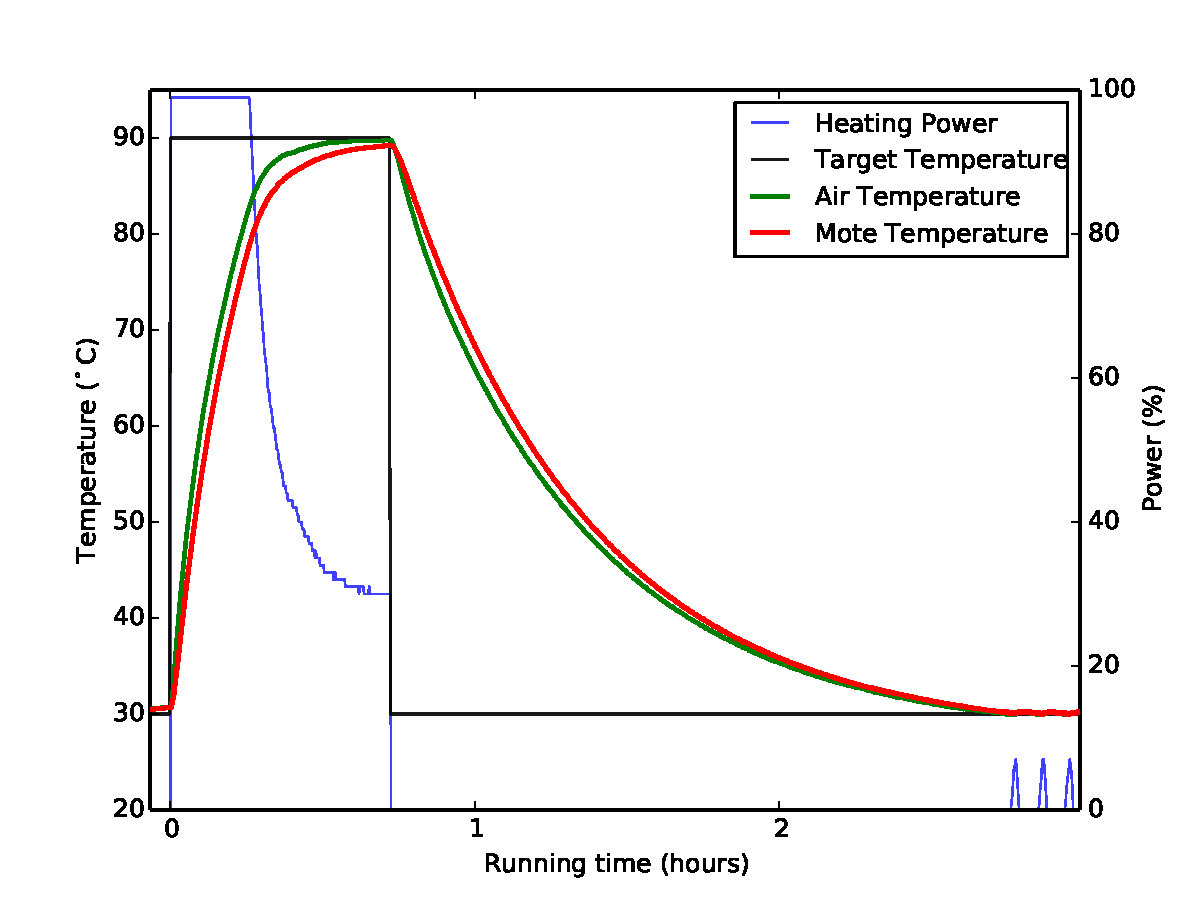
\includegraphics[width=1\columnwidth]{figures/box_heating_cooling}
	\caption{Temperature box heating up to $90\,^{\circ}\mathrm{C}$, then cooling back down to $30\,^{\circ}\mathrm{C}$.}
    \label{fig:box_heating_cooling}
\end{figure}

\begin{figure}[t]
	\centering
    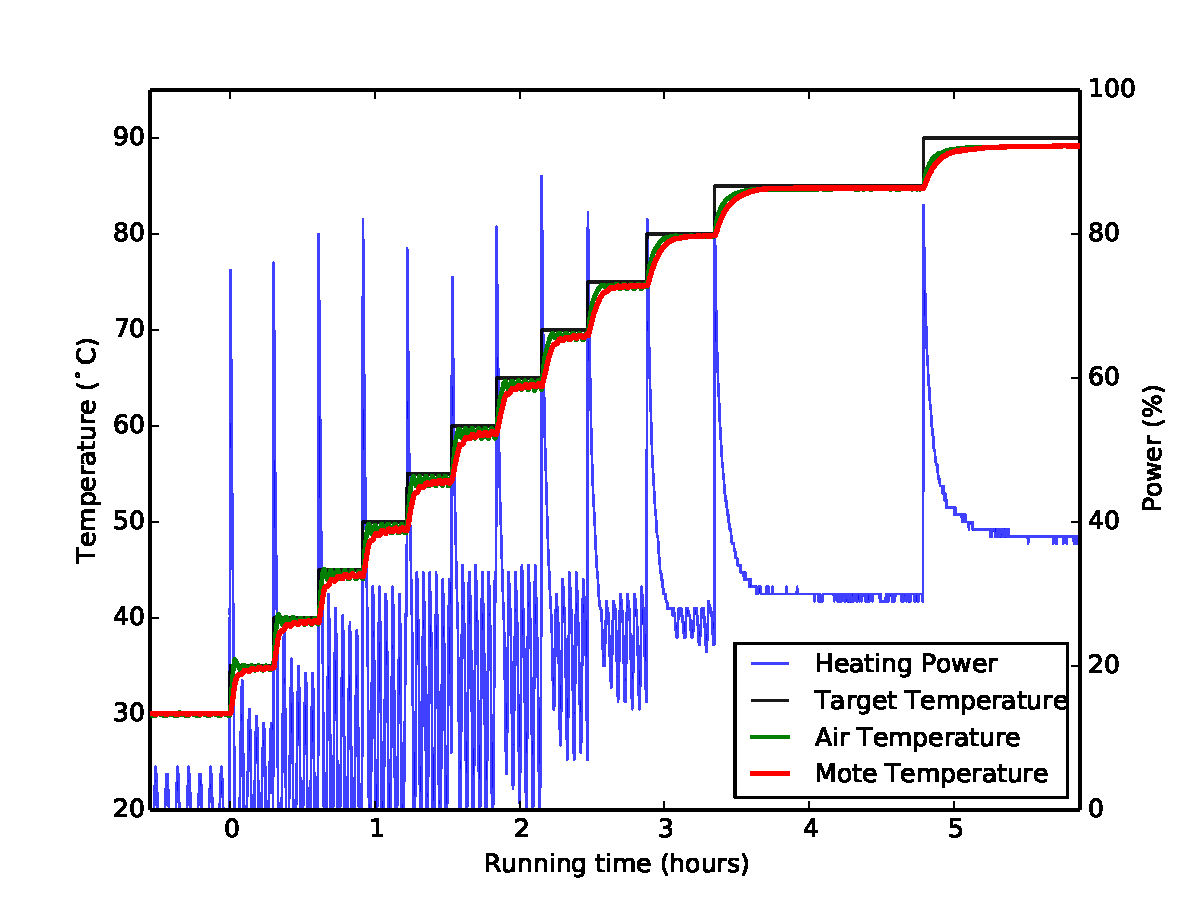
\includegraphics[width=1\columnwidth]{figures/box_heating_step}
	\caption{Typical experiment setup with temperature increases in steps of $5\,^{\circ}\mathrm{C}$.}
    \label{fig:box_heating_step}
\end{figure} 
\chapter{Experiments}

Several experiment setups were designed to focus on the effect of temperature on the mote hardware and link quality.
All experiments were done using the on-board PCB antenna, sending on channel 26 to minimize WiFi interference.

\section{Clock Drift}

The Tmote Sky uses a MSP430 microcontroller clocked an integrated ring oscillator called the \ac{DCO}.
Since the generated clock frequency varies with temperature, voltage and from chip-to-chip, the \ac{DCO} can be fine-tuned using a modulation functionality.
During booting, TinyOS calibrates the \ac{DCO} using the external low-current 32.756Hz watch crystal to generate a more accurate 1MHz clock.
It should be noted, that calibration only occurs after a reset, and not periodically during program execution.

We noticed a problem, where serial communication stopped working after heating the nodes above $55-60\,^{\circ}\mathrm{C}$. Below this temperature the problem could be mitigated by resetting the mote to trigger a recalibration of the \ac{DCO}.
We therefore looked at the output of the \ac{UART} module with a logic analyzer and measured the how the selected baudrate changes over temperature.
Since the baudrate is generated by scaling the \ac{DCO}, relative baudrate error is equivalent to relative \ac{DCO} error.
Figure~\ref{fig:baudrate_error} shows the relative error of four baudrates over temperature.
We calculate an average temperature clock drift coefficient of $-0.367\%/\,^{\circ}\mathrm{C}$, which is within the typical range according to the datasheet. Similar coefficients were found by Z{\'u}{\~n}iga~\etal~\cite{Zuniga2013}.

\begin{figure}[t]
	\subfigure[Relative error of four baudrates.] {
    	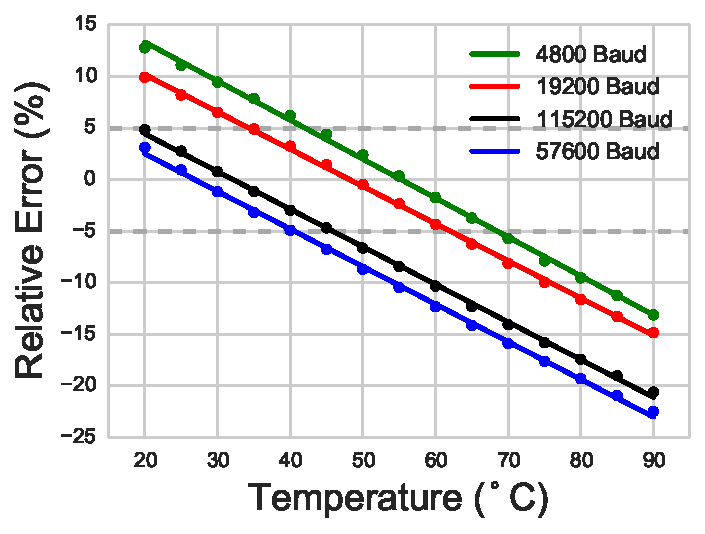
\includegraphics[width=0.5\columnwidth]{figures/baudrate_error}
    	\label{fig:baudrate_error}
    }
    \subfigure[Relative error of \acs{DCO} calibration.] {
	    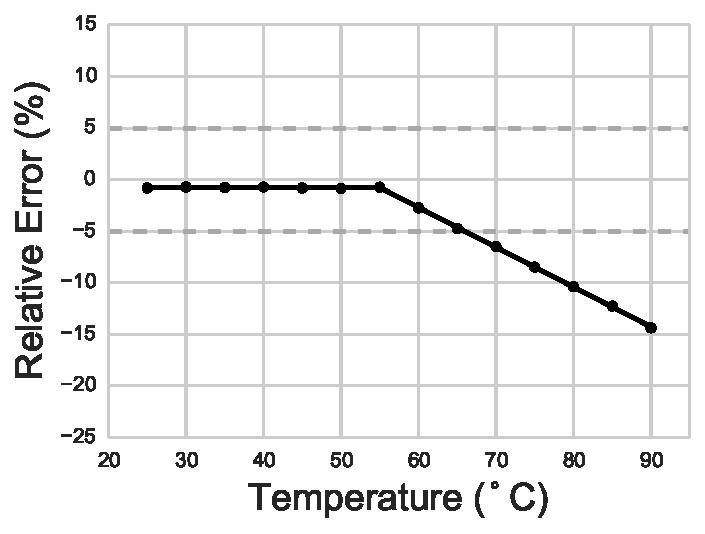
\includegraphics[width=0.5\columnwidth]{figures/reboot_dco_drift}
	    \label{fig:reboot_drift}
	}
	\subfigure[Relative error of corrected baudrate.] {
	    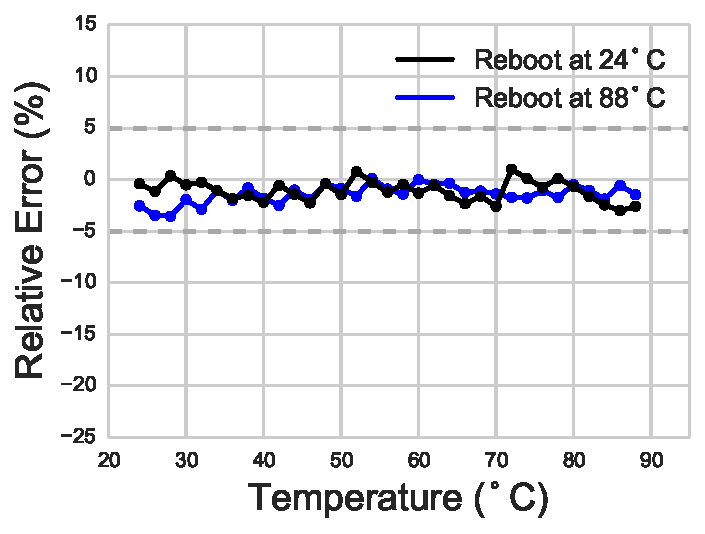
\includegraphics[width=0.5\columnwidth]{figures/baudrate_correction_error}
	    \label{fig:baudrate_look_up_error}
	}
	\subfigure[Values of baudrate correction look-up table.] {
	    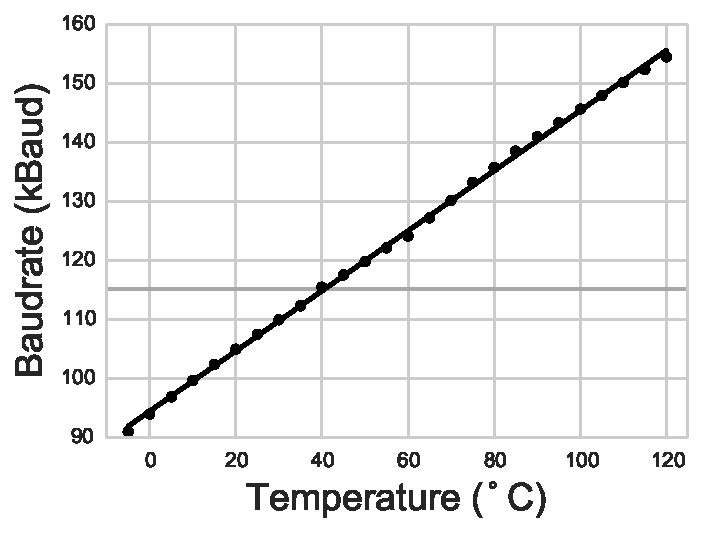
\includegraphics[width=0.5\columnwidth]{figures/baudrate_correction_table}
	    \label{fig:baudrate_look_up}
	}
	\caption{\acs{UART} and \acs{DCO} calibration errors vs. temperature. Note that \acs{UART} can tolerate up to $\pm5\%$ error.}
\end{figure}

We then measured the relative baudrate error after rebooting over temperature.
As shown in Figure~\ref{fig:reboot_drift}, the TinyOS implementation of the \ac{DCO} calibration only works until $55\,^{\circ}\mathrm{C}$, after which it has no corrective effect on CPU frequency, making periodic \ac{DCO} calibration during program execution ineffective.

We chose not to correct clock drift directly, but counteract the effect on baudrate, by creating a lookup-table of ``inverse'' correction baudrates for 115.2kbps and applying it with temperature as shown in Figure~\ref{fig:baudrate_look_up}.
Since calculation of prescaler values at runtime is costly, the look-up table contains precalculated values, which are then copied into the registers at runtime.
The on-board sensor provides temperature to the \ac{UART} module which then selects new prescaler values from the look-up table for every $5\,^{\circ}\mathrm{C}$, which shows as a sawtooth pattern in the resulting relative error of the corrected baudrate as shown in Figure~\ref{fig:baudrate_look_up_error}.

Note that the receiver can still correctly read serial data if the relative error does not deviate more than $\pm5\%$. During reception the falling edge of the startbit is used to synchronize the sampling points of all bits and with 8 databits, 1 startbit and 1 stopbit (8N1 configuration), the stopbit must be sampled during the last $10\%$ of reception time, hence an error tolerance of $\pm5\%$.
For example, the tolerance for 7-bit transfers (9 baudtimes) increases to $\pm5.56\%$.

\todo{last paragraph is a bit cryptic. Overthink it.}

\section{Bit Error Patterns}

We designed two experiments to investigate the results of Schmidt~\etal~\cite{Schmidt2013}, in particular the effect of temperature and hardware revision on bit error distribution.

\subsection{Effects of board layout}
\label{subsec:effects_of_board_layout}

While both versions we used are drop-in replacements for the Telos design devised by Polastre~\etal~\cite{Polastre2005}, the newer MTM-CM5000 version uses a slightly different schematic and different board layout.
Notable differences include the 3V voltage regulator and the layout of the radio circuitry.

In the experiment a pair of CM5000 and original motes transmitted to two CM5000 and two original motes.
This redundant placement shown in Figure~\ref{fig:8_mote_setup} was chosen so that the same transmission was received by both types.
Over the course of six days the four transmitters sent 563.500 messages each, totalling 2.254.000 transmitted messages at power setting 2. Of those transmitted messages a total of 5.280.369 messages were received, 2.497.744 of which had at least one bit error.
The experiment was located in a large climate-controlled server room in the basement, therefore the temperature remained within $20-25\,^{\circ}\mathrm{C}$ with no other changes in the environment.

\begin{figure}[H]
	\centering
	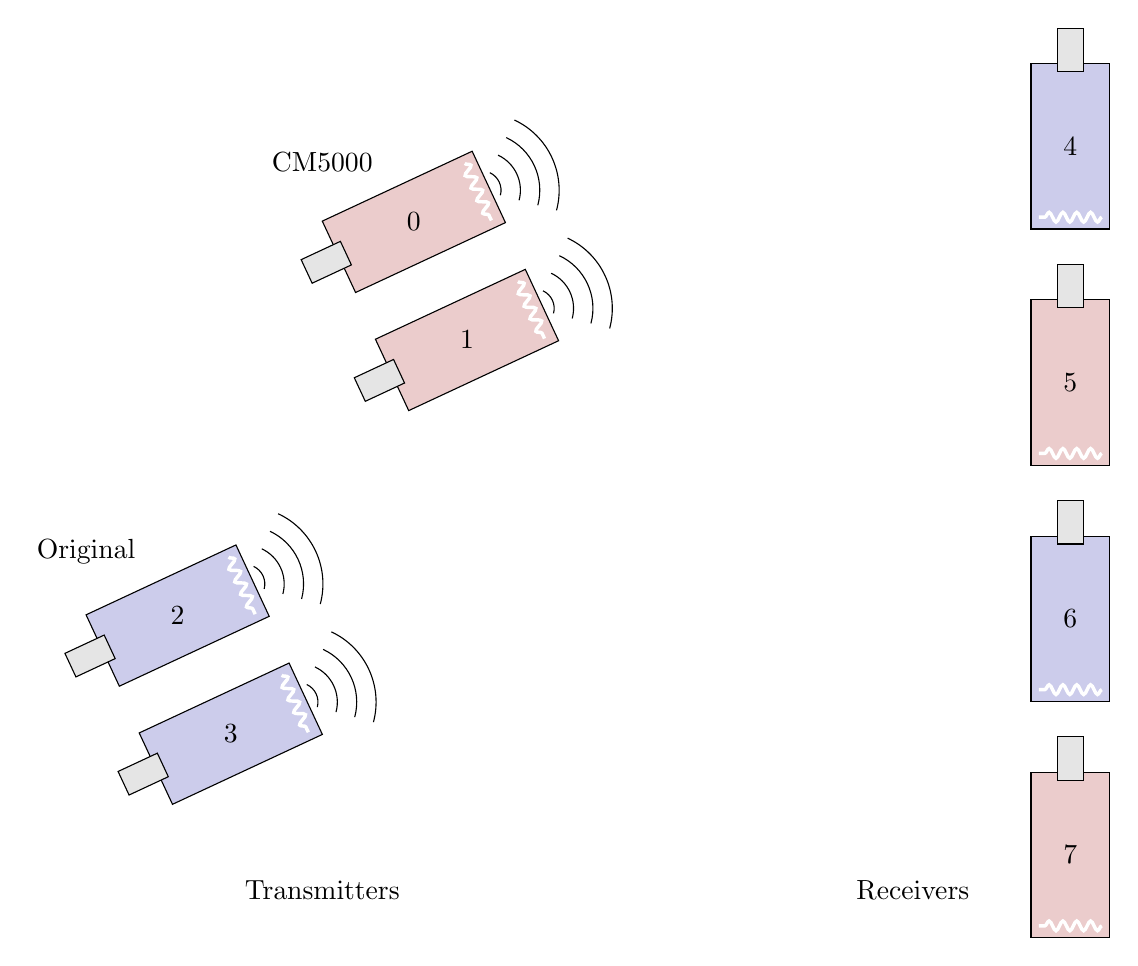
\begin{tikzpicture}
		\newcommand\receiver[5]{%
		    \begin{scope}[xshift=#1cm,yshift=#2cm,rotate=#3]
		        \draw[fill=#4] (0,0) rectangle (1,2.1);
		     	\draw[fill=black!10] (0.33,0.1) rectangle (0.66,-0.45);
		     	\draw[snake=snake, white, segment amplitude=1.75, segment length=5, line width=1.25pt] (0.1, 1.95) -- (0.9, 1.95);
		     	\node at (0.5cm, 1.05cm) {#5};
		    \end{scope}
		}
		\newcommand\transmitter[5]{%
			\receiver{#1}{#2}{#3}{#4}{#5};
		    \begin{scope}[xshift=#1cm,yshift=#2cm,rotate=#3]
		     	\draw[snake=expanding waves, segment angle=40, segment length=7] (0.5,2) -- (0.5,3);
		    \end{scope}
		}

		% new = red, old = blue
		% new transmitter
		\transmitter{3}{7}{-65}{motered}{0};
		\transmitter{3.675}{5.5}{-65}{motered}{1};		

		% new transmitter
		\transmitter{0}{2}{-65}{moteblue}{2};
		\transmitter{0.675}{0.5}{-65}{moteblue}{3};

		\receiver{13}{0}{180}{motered}{7};
		\receiver{13}{3}{180}{moteblue}{6};
		\receiver{13}{6}{180}{motered}{5};
		\receiver{13}{9}{180}{moteblue}{4};

		% labels
		\node at (3, 7.75) {CM5000};
		\node at (0, 2.8) {Original};

		\node at (3, -1.5) {Transmitters};
		\node at (10.5, -1.5) {Receivers};
	\end{tikzpicture}
	\caption{Experiment setup from above with four transmitters and receivers.}
	\label{fig:8_mote_setup}
\end{figure}

Note that the CM5000 motes required to be physically closer to the receivers at the same power setting to have similar link quality as the original motes.
This might be hinting at a difference in range between the two hardware layouts, however, our experiment was not setup to systematically investigate range.

In the initial evaluation we noted some significant differences in the quality of some links, were the co-located transmitters are sending to the same receiver.
For example, the link 3-5 is of very good quality with over 99\% PRR, however link 2-5 shows quite the opposite with less than 1\% PRR, even though both transmitters a located at the same distance and angle from the receiver.
This confirms the findings of Baccour~\etal~\cite{Baccour2012}, specifically that link quality is anisotropic, \ie the communication range exhibits a nonspherical pattern.
More exhibitions of this behavior can be found in the complete table of link qualifiers in the Appendix as Table~\ref{tab:8mote_link_qualities}.

Further analysis revealed the same bit and symbol error patterns as first discovered by Schmidt~\etal~\cite{Schmidt2013}, which state that within any transmitted symbol, the first three MSB are more likely to break than the LSB and that symbols with the MSB set to 1 (\ie 0x8 to 0xF) are more likely to brea.
The probability of bit errors are plotted in Figure~\ref{fig:8mote_bit_errors}, with the first 12 bytes (96 bits) consisting of the message header with partially fixed content and the remaining 80 bytes are the constant payload, made up of two 32 byte patterns of 0x0000, 0x1111, ..., 0xFFFF, and one 16 byte pattern of 0x00, 0x11, ..., 0xFF.

\begin{figure}[H]
	\subfigure[XL symbol influence.] {
    	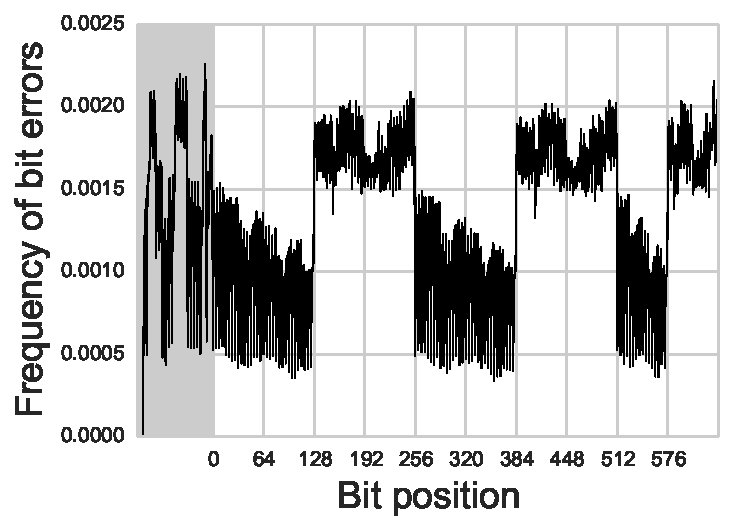
\includegraphics[width=0.5\columnwidth]{figures/8mote_0-5_xor}
    	\label{fig:8mote_bit_errors_xl}
    }
    \subfigure[L symbol influence] {
	    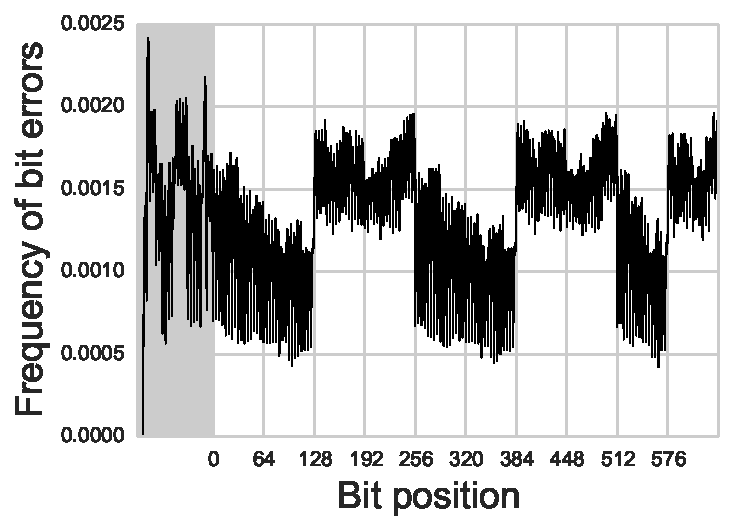
\includegraphics[width=0.5\columnwidth]{figures/8mote_1-6_xor}
	    \label{fig:8mote_bit_errors_l}
	}
	\subfigure[M influence.] {
	    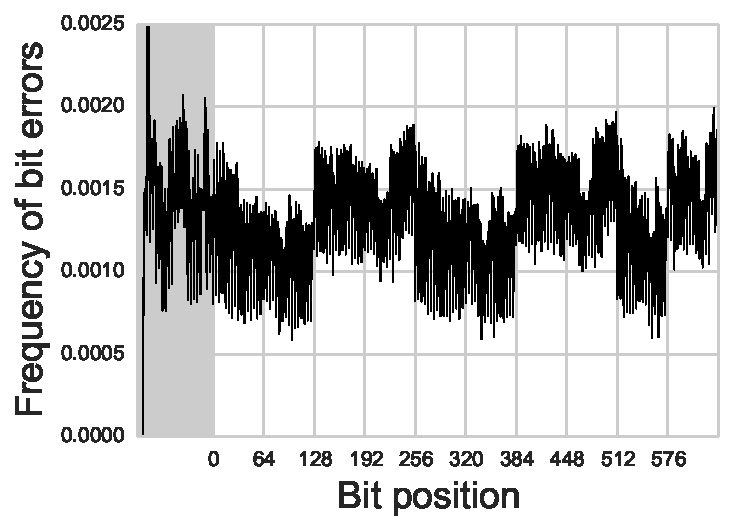
\includegraphics[width=0.5\columnwidth]{figures/8mote_2-6_xor}
	    \label{fig:8mote_bit_errors_m}
	}
	\subfigure[S influence.] {
	    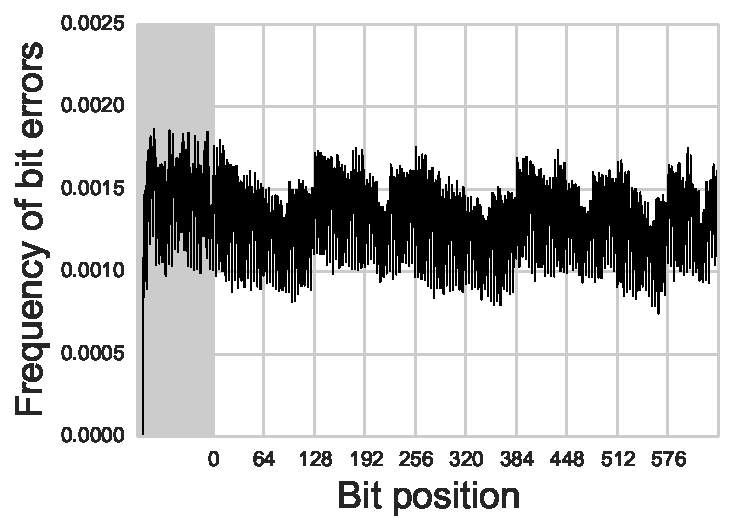
\includegraphics[width=0.5\columnwidth]{figures/8mote_2-7_xor}
	    \label{fig:8mote_bit_errors_s}
	}
	\caption{Four magnitudes of symbol content influence on bit error pattern.}
	\label{fig:8mote_bit_errors}
\end{figure}

We were able to confirm the findings of Schmidt~\etal{} and extend them with a classification of the influence of symbols on bit error probability.
The subfigures show four magnitudes of this phenomenon, ranging from and extreme to almost no difference between symbols, named XL, L, M and S.
The remaining links can be classified into these four categories as done in Table~\ref{tab:8mote_bit_error_link_classification}.

\begin{table}[H]
	\begin{tabularx}{\linewidth}{|c*{4}{|c}|}
	\hline
	\T \cellcolor{slightgray} Receiver	& \multicolumn{1}{X|}{\cellcolor{motered} \centering Sender 0} & \multicolumn{1}{X|}{\cellcolor{motered} \centering Sender 1} & \multicolumn{1}{X|}{\cellcolor{moteblue} \centering Sender 2}	& \multicolumn{1}{X|}{\cellcolor{moteblue} \centering Sender 3}\\
	\hline

	\cellcolor{moteblue}\T 4 & S  & n/a & n/a & n/a \B\\
	\hline
	\cellcolor{motered}\T  5 & XL & XL  & L   & XL  \B\\
	\hline
	\cellcolor{moteblue}\T 6 & XL & L   & M   & n/a \B\\
	\hline
	\cellcolor{motered}\T  7 & L  & n/a & S   & L   \B\\
	\hline 
	\end{tabularx}

	\caption{Classification of all links with enough bit errors (otherwise marked with n/a).}
	\label{tab:8mote_bit_error_link_classification}
\end{table}



\chapter{Simulation of Bit Error Patterns}

Considering the difficulty of replicating the exact link twice, we wrote a simple trace-based simulator that allows to apply the same bit error pattern from a real experiment onto new payload link-by-link.
This way we can keep the temporal variations of the link intact and single out the effect of bit error patterns on different payloads.

In this chapter we will describe how we model the patterns described in Section~\ref{sec:bit_error_patterns} to simulate them on new payload, and what the limitations of this method are.

\section{Design}

The simulator gets its bit error configuration from a log of a real world experiment, and re-runs this experiment link-by-link but using different payload.
We only simulate bit error patterns, all other properties of the link, such as link qualifiers, temperature, transmission power, are copied from the original link.
If a link was not received by a receiver, we do not simulate this link, but register the timeout.
This makes later comparison of the simulated results with the real experiments much easier.

\todo{Add design visualization.}

\subsection{Pattern extraction}

For every original link in the experiment log, we count the bit errors per bit per symbol.
This results in a table of 16 symbols, each of which has 4 entries, one for every bit in the symbol.
The table is then normalized for the occurrence of the respective symbol to yield a relative bit error occurrence per symbol for this specific link.

This table can be averaged over several links using a sliding window, which reduces noise and increases probability of seeing all symbols with their respective bit error patterns.
Note, that this creates a table of \emph{average} bit error probabilities per symbol over one or several links.
Therefore we also collect the distribution of bit error burst length over this window.

\subsection{Pattern application}

Every logged link, consisting out of transmitted and received messages, is copied and its transmitted payload replaced by a new payload.
Then a corruption pattern is generated by randomly corrupting each new symbol with the probability defined in the bit error table.
This corruption pattern consists mostly out of single bit errors, therefore for every single bit error, we randomly stretch it in length proportionately to the burst error distribution of the original link.
The corruption sequence is applied to the transmitted payload and written to the received message of the copied link.

\subsection{Limitations}

We map bit error distribution per symbol, therefore every symbol must be available in the original payload for this table to be complete.
Experiment logs with constant payload in which not every symbol is available should be avoided.
For random payload our payload size of 93 bytes yields 186 symbols, for which it is unlikely to not see every 16 symbols at least once.

Another limitation is our modeling of bit error burstiness.
By ``simply'' applying the collected bit error table by symbol onto new payload, we are effectively interleaving the original burst errors and therefore obscuring this property of the original link.
With our simple simulation, we can only add burst errors to correct for relative occurrence compared to the original frame, but not willfully ``place'' these burst errors at the correct position to achieve the distinct burst error properties of the original link.


\section{Accuracy}

To evaluate the performance of the simulator, we used the experiment traces containing constant payloads as well as random payloads.
By tuning the link input window size and the aggression of the burst error generator, we were able to replicate similar enough bit error patterns for our purposes.
We found best accuracy with a window size of two links and two passes of the burst generator.

Subfigure~\ref{fig:8mote_xl_xor_simulation} and \ref{fig:8mote_s_simulation} show the bit error pattern resulting of simulating XL and S magnitudes of the experiment described in Subsection~\ref{subsec:effects_of_board_layout}.
Compared to the original patterns in Figure~\ref{fig:8mote_bit_errors}, the simulation generates a less noisy footprint with less amplitude, which makes the differences in symbols clearly visible.
This is, of course, due to the averaging during the symbol error construction which is accompanied with the smoothing of these values.

The limitations of our burst error modeling clearly show in the burst error graph in Figure~\ref{fig:8mote_xl_burst_simulation} of the simulation. In comparison to Figure~\ref{fig:8mote_burst_error}, the simulated corruption does not exhibit the drop between 4/5-bit and 8/9-bit bursts and generates longer bursts more frequently, but at least the distribution is the same between the two magnitudes.

\begin{figure}[t]
	\subfigure[Simulated XL bit error pattern.] {
		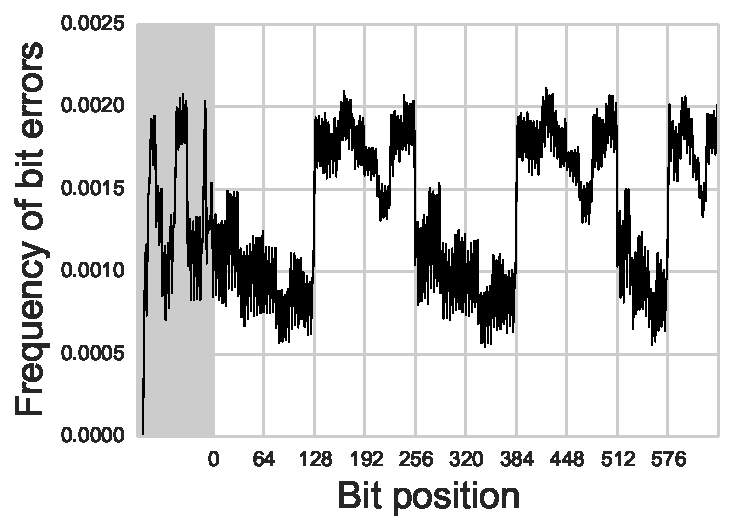
\includegraphics[width=0.5\columnwidth]{figures/8mote_0-5_xor_simulation}
		\label{fig:8mote_xl_xor_simulation}
	}
	\subfigure[Simulated S bit error pattern.] {
		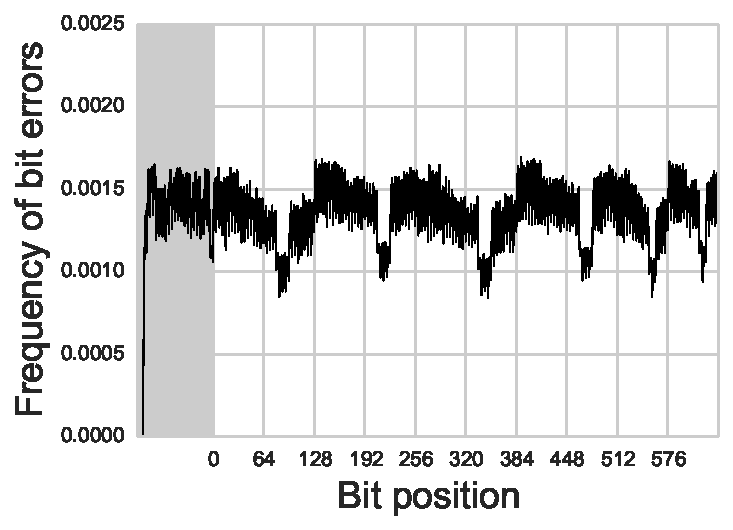
\includegraphics[width=0.5\columnwidth]{figures/8mote_2-7_xor_simulation}
		\label{fig:8mote_s_simulation}
	}
	\subfigure[Simulated XL burst error length.] {
		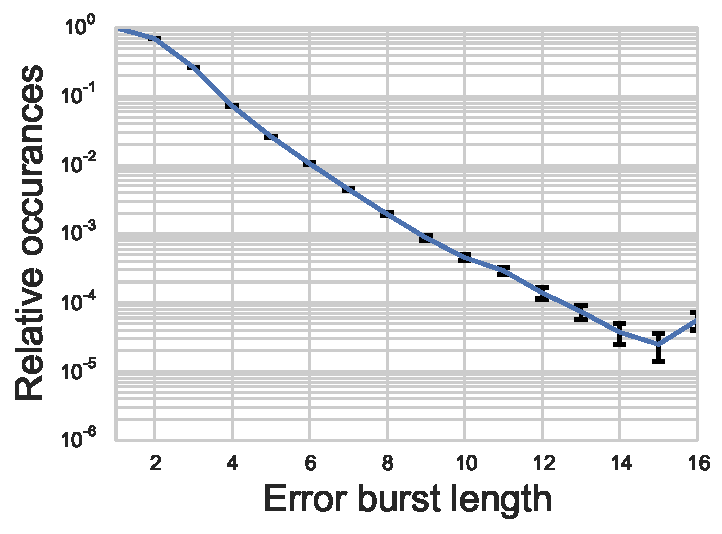
\includegraphics[width=0.5\columnwidth]{figures/8mote_0-5_burst_simulation}
		\label{fig:8mote_xl_burst_simulation}
	}
	\subfigure[Simulated S burst error length.] {
		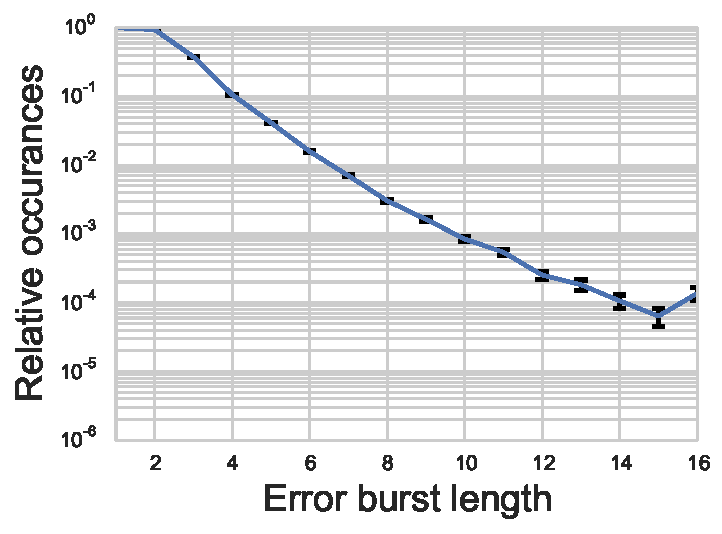
\includegraphics[width=0.5\columnwidth]{figures/8mote_2-7_burst_simulation}
		\label{fig:8mote_s_burst_simulation}
	}
	\caption{Error patterns of simulated constant payload using traces with constant payload.}
	\label{fig:8mote_bit_errors_simulation}
\end{figure}

For accurate results we also need to compare the overall number of bit errors of the original with the simulated link.
For this we plot the normalized \ac{PRR} of a real experiment with random message payload and the simulation of that experiment with new random payload as shown in Figure~\ref{fig:prr_simulation_comparison}.
The simulation follows the shape of the original \ac{PRR} well, however, seems to have more variation in the number of error-free receptions shown as the black line.
Note that the timeouts shown in grey are the same for the simulation, since they are copied from the original.

\begin{figure}[t]
	\subfigure[Original 1-0] {
		\includegraphics[width=0.475\columnwidth]{figures/simulation_prr_original_0}
		\label{fig:prr_simulation_original_0}
	}
	\subfigure[Original 0-1] {
		\includegraphics[width=0.475\columnwidth]{figures/simulation_prr_original_1}
		\label{fig:prr_simulation_original_1}
	}
	\subfigure[Simulation 1-0] {
		\includegraphics[width=0.475\columnwidth]{figures/simulation_prr_simulation_0}
		\label{fig:prr_simulation_simulated_0}
	}
	\subfigure[Simulation 0-1] {
		\includegraphics[width=0.475\columnwidth]{figures/simulation_prr_simulation_1}
		\label{fig:prr_simulation_simulated_1}
	}
	\caption{Original and simulated \acs{PRR} of two links of the same experiment over time.}
	\label{fig:prr_simulation_comparison}
\end{figure}

These results show that this simple simulator is a very good time- and cost-saving alternative method to testing the effects of different payloads over a certain link, if good original data is available.
Using our trace-based simulator eliminates the effect of uncontrollable environmental factors or hardware issues on repeatability and allows us to focus purely on the message content, without assuming a completely idealistic and monolithic link simulation.






















\chapter{\acl{FEC}}
\label{chap:forward_error_correction}

In the last chapters, we described the effect of temperature on \ac{BER} patterns and \ac{PRR}, without drafting any specific recommendations how to improve this loss of link quality.
\ac{FEC} is a well known technique to improve throughput in links of poor quality, however, once a \ac{ECC} and its parameters have been chosen, usually they remain static and do not change over time.
This means that for links where the quality is not stable over time, as in \acp{WSN}, the chosen \ac{ECC} incurs unneeded overhead in links with overal good link quality, and underperforms in links with poor quality.

We therefore wanted to investigate how using temperature as an indicator for adapting \ac{ECC} parameter can benefit \ac{PRR} and throughput and what improvements and limitations to expect.
In doing so, we are moving away from a macro-view of all influences on link quality to focus on the impact of temperature on \ac{FEC} on \emph{one} link at a time.

We extended the control software described in Section~\ref{sec:control_software} to encode messages to be sent and to decode received messages with an \ac{FEC} scheme.
The messages are logged in the same format, with the additional information of the FEC scheme and coding strength.
This allows us to reuse our existing evaluation software to easily map error-free \ac{PRR} to \emph{decoded} error-free \ac{PRR}.


\section{Choice of \acs{FEC} Scheme}

Choosing a coding scheme is not only a matter of its error correction capabilities, but also about the complexity of its coder and decoder, considering the tight computational resources of a \ac{WSN} mote.
Practical implementations are therefore limited to cyclic linear block coding, with the most widely used codes being binary \ac{BCH} and non-binary \ac{RS} codes, which can be combined with interleaving and code shortening~\cite{Liu1997}.
Furthermore, since data payload size is limited to 125 bytes by the \ac{MPDU}, of which we use 93 in our messages (with 80 bytes data), a low coding overhead among \ac{ECC}s with the same error correction capability is preferred.

A \ac{RS} code works over $m$-bit symbols, and is denoted as $RS(n, k)$, where $n$ is the number of $m$-bit symbols in a codeword, and $k$ the number of original $m$-bit data symbols.
This leaves $n-k$ parity $m$-bit symbols, as shown in Figure~\ref{fig:rs_codeword}.
The symbol size $m$ can be set to bit-level, byte-level or packet-level size. We will use byte-level ($m=8$) symbol sizes, since they are efficient to work with on a microcontroller.
A \ac{RS} decoder can correct up to $t=(n-k)/2$ symbol errors, and up to $2t$ erasures, if the positions of the symbol errors are known~\cite{Liu1997}.

Similarly, for symbol size $m \ge 3$ and symbol error occurance $t < 2^{m-1}$, a \ac{BCH} code encodes block lengths of $n = 2^m - 1$ bit with $n-k \le mt$ parity check bits by multiplication with a generator matrix, that contains a $n \times n$ identity and a $n \times (n-k)$ binary matrix.
The decoder can construct a parity matrix using this information, which allows correction of $t$-bit errors, depending on the parameters chosen~\cite{Liu1997}.

Since the \ac{RS} scheme works by correcting entire $m$-bit symbols ($m=8$ for our case), burst errors up to $m$-bit in the same symbol require only correcting this specific symbol, while one-bit errors in many different symbols requires correcting all of these symbols.
\ac{RS} codes therefore perform better than \ac{BCH} codes in conditions with burst errors as described in Subsection~\ref{subsec:effects_of_board_layout}, but worse if same amount of bit errors are spread around more independently.
The performance of \ac{BCH} codes can be improved however, by interleaving symbols after encoding before transmission, which spreads out burst errors into many single bit errors.
However, \ac{BCH} codes generally require more transmission overhead compared with \ac{RS} codes of the same error correction capabilities.

\ac{RS} codes are well understood coding schemes, which have been compared to many others.
By using \ac{RS} codes as a benchmark we enable application of our results onto other, more complex schemes, such as a modified Turbo Code~\cite{Schmidt2009} and \ac{LDPC}~\cite{Sartipi2004} codes, which have been shown to outperform cyclic linear block codes.
Furthermore, a \ac{RS} implementation optimized for TinyOS, called TinyRS~\cite{Liang2010}, exists and therefore does not need to be implemented manually.

\begin{figure}[t]
	\begin{tikzpicture}[>=stealth', |<->|, very thick, shorten <=-0.5pt, shorten >=-0.5pt]

		\draw[thick] (0,-0.35) rectangle (10,0.35) node[midway] {Data};
		\draw[fill=slightgray, thick] (10,-0.35) rectangle (15,0.35) node[midway] {Parity};

		\draw (0,0.7) -- (10,0.7) node[midway, above] {$k$};
		\draw (10,0.7) -- (15,0.7) node[midway, above] {$80 - k$};
		\draw (0,-0.7) -- (15,-0.7) node[midway, below] {$n = 80$};

	\end{tikzpicture}
	\caption{Structure of an $RS(n, k)$ encoded codeword of 80 bytes length.}
	\label{fig:rs_codeword}
\end{figure}

\section{\acs{RS} Scheme Simulation}
\label{sec:fec_scheme_simulation}

To be able to investigate the effect that different \ac{RS} coding strengths have on decoded \ac{PRR}, we needed a way to compare experiment results.
Due to the difficulty of recreating the \emph{exact} same conditions for several series of real world experiments, we chose to create and use a trace-based simulator to apply the bit error patterns of an original experiment onto several new $RS(n, k)$ encoded random payloads.

By interpreting the $RS(80, 70)$ encoded random payload as pseudo-random in the context of Section~\ref{sec:packet_reception_rate}, we made dual-use of that experiment.
This allows us an in-depth description of the link conditions onto which we built our analysis of \ac{RS} performance.

We will next describe how we use the raw data of this experiment as an input for our simulation, by extracting its \ac{BER} patterns and applying them onto new payload, and discuss accuracy and limitations.

\subsection{Design}

The simulator re-runs an original experiment message-by-message over its log, and outputs a new one.
We only simulate \ac{BER} patterns, all other properties of the link, such as link qualifiers, temperature, transmission power, are copied from the original link, as visualized in Figure~\ref{fig:simulator_design}.
In addition, if a message was not received by a receiver, we simply preserve it as a timeout, to make later comparison of the simulated results with the real experiments much easier.

Our simulator also works with experiments where a transmitted message is received by multiple receivers as in Section~\ref{subsec:effects_of_board_layout}.
In such a case, the simulator will apply its algorithm to every received message.

\begin{figure}[t]
	\centering
	\tikzset{
	    %Define standard arrow tip
	    >=stealth',
	    %Define style for boxes
	    punkt/.style={
	           rectangle,
	           rounded corners,
	           draw=black, very thick,
	           text width=2cm,
	           minimum height=1cm,
	           text centered},
	    % Define arrow style
	    pil/.style={
	           ->,
	           very thick,
	           shorten <=2pt,
	           shorten >=2pt,}
	}
	\begin{tikzpicture}

		\fill[color=slightgray, rounded corners] (1.4,-4) rectangle (11,-2);

		\node[punkt] (input) {Input Message(s)};
 		\node[punkt, right=0.8cm of input] (parser) {Parser};
 		\node[punkt, right=3.85cm of parser] (formatter) {Formatter};
 		\node[punkt, right=0.8cm of formatter] (output) {Output Message};

 		\node[punkt, below=2cm of parser, fill=white] (analyzer) {Analyzer};
 		\node[punkt, below=2cm of formatter, fill=white] (corruptor) {Corrupter};
 		\node[right=0.85cm of corruptor] (payload) {New Payload};

 		\draw[pil] (input) -- (parser);
 		\draw[pil] (parser) -- (formatter) node[midway, below] {LQI, RSSI};
 		\path (parser) -- (formatter) node[midway, above] {Temperature};
 		\draw[pil] (formatter) -- (output);

 		\draw[pil] (parser) -- (analyzer) node[midway, left] {Original Payload(s)};
 		\draw[pil] (analyzer) -- (corruptor) node[midway, above] {BER pattern};
 		\draw[pil] (payload) -- (corruptor);
 		\draw[pil] (corruptor) -- (formatter) node[midway, right] {New Corrupted Payload};

 		\draw[pil] (input) edge[bend left=25] node[below]{Timeout} (output);

		% \draw (-1.2,-5) rectangle (13.8,1);
	\end{tikzpicture}
	\caption{Schematic design of our trace-based simulator: the payloads of multiple original messages can be analyzed to extract the \ac{BER} pattern, which is then applied to new payload.}
	\label{fig:simulator_design}
\end{figure}


\paragraph{Pattern Extraction}

Since we know that the \ac{BER} pattern is different for every of the 16 4-bit symbols, we need to generate a corruption probability for each bit within every symbol.
For that we sum up the bit errors per bit \emph{per symbol} for every original received message in the experiment in a corruption table.
The corruption table is then normalized for the occurrence of the respective symbol in the original message to yield a relative bit error occurrences \emph{per symbol} for this specific link.

This table can be averaged over several links using a sliding window, which reduces noise and increases the likelihood of seeing all symbols with their respective bit error patterns at least once.
This will create a corruption table of \emph{average} bit error probabilities per symbol over one or more messages.
We also average the distribution of bit error burst lengths over these messages in a burst error table.
Both the corruption and the burst error table will then be handed over to the corruption generator.

Since these tables are generated on-the-fly entirely from an experiment log, even the anomalous patterns described in Section~\ref{subsec:pattern_anomalies} can be extracted.

\paragraph{Pattern Application}

A corruption pattern is generated by randomly corrupting each new symbol with the probability defined in the bit error table.
This corruption pattern needs to be adapted for the burst error distribution of the original message by lengthening single bit errors accordingly.

The corruption sequence is applied to the new payload defined by us and written out as a new received message of the original link.

\paragraph{Limitations}

Since we map and apply bit error distribution \emph{per symbol}, every symbol must be available in the original payload at least once for this table to be complete.
Experiment logs with constant payload in which not every symbol is available should be avoided.
For random payload our message size of 93 bytes yields 186 symbols, for which it is unlikely to not see every 16 symbols at least once.

Another limitation is our modeling of the burst error distribution.
By ``simply'' applying the collected bit error table by symbol onto new payload, we are effectively interleaving the original burst errors and therefore obscuring this property of the original link.
With our simple simulation, we can only add burst errors to correct for relative occurrence compared to the original frame, but not willfully ``place'' these burst errors at the correct position to achieve the distinct burst error properties of the original link.

\subsection{Accuracy}
\label{subsec:simulation_accuracy}

To evaluate the performance of the simulator, we ran it on experiment traces containing constant payloads as well as $RS(80,70)$ encoded payloads.
By tuning the link input window size and the burst error generator, we were able to replicate similar enough bit error patterns for our purposes.
We found best accuracy with a window size of two messages.

\paragraph{Bit Error Distribution Patterns}

Figure~\ref{fig:8mote_xl_xor_simulation} and \ref{fig:8mote_s_simulation} show the bit error pattern resulting of simulating XL and S magnitudes of the experiment described in Subsection~\ref{subsec:effects_of_board_layout}.
Compared to the original patterns in Figure~\ref{fig:8mote_bit_errors}, the simulation generates a less noisy footprint with less amplitude, which makes the differences in symbols clearly visible.
This is, of course, due to the averaging during the symbol error construction that is accompanied with the smoothing of these values.

\paragraph{Burst Error Distribution}

The limitations of our burst error modeling clearly show in the burst error graph in Figure~\ref{fig:8mote_xl_burst_simulation} of the simulation. In comparison to Figure~\ref{fig:8mote_burst_error}, the simulated corruption does not exhibit the drop between 4/5-bit and 8/9-bit bursts and generates longer bursts more frequently.

\begin{figure}[t]
	\subfigure[Simulated XL bit error pattern.] {
		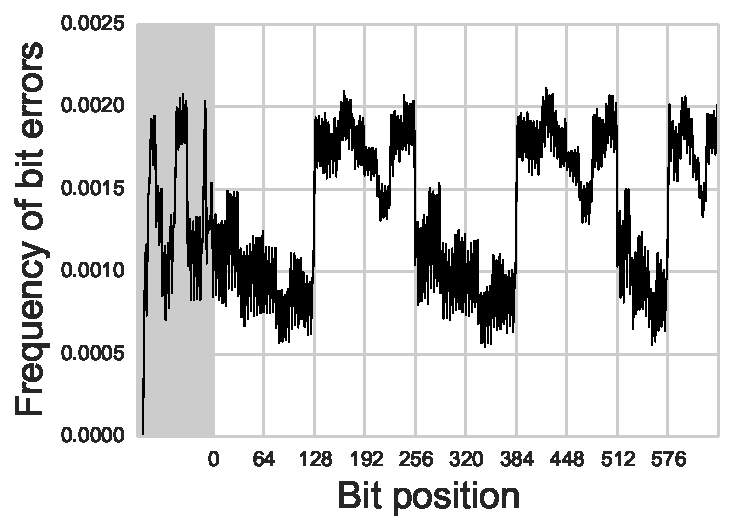
\includegraphics[width=0.475\columnwidth]{figures/8mote_0-5_xor_simulation}
		\label{fig:8mote_xl_xor_simulation}
	}
	\subfigure[Simulated S bit error pattern.] {
		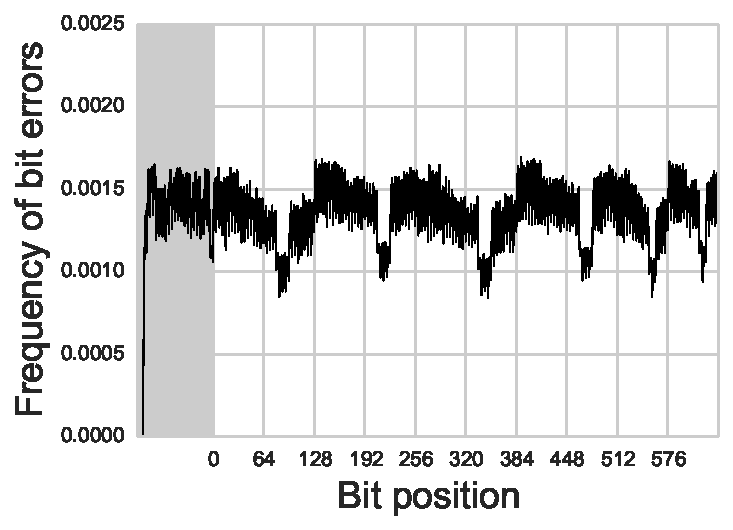
\includegraphics[width=0.475\columnwidth]{figures/8mote_2-7_xor_simulation}
		\label{fig:8mote_s_simulation}
	}
	\subfigure[Simulated XL burst error length.] {
		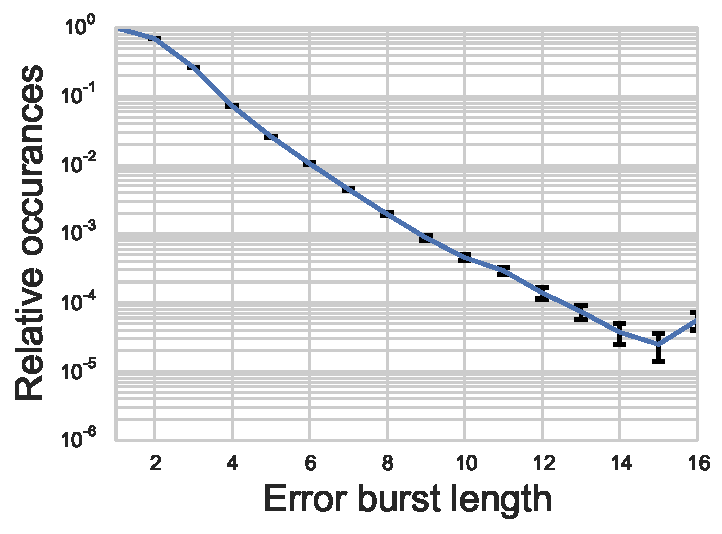
\includegraphics[width=0.475\columnwidth]{figures/8mote_0-5_burst_simulation}
		\label{fig:8mote_xl_burst_simulation}
	}
	\subfigure[Simulated S burst error length.] {
		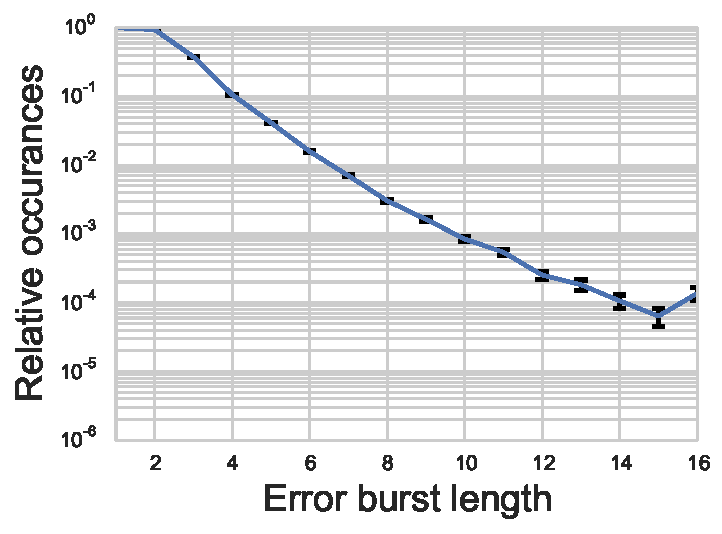
\includegraphics[width=0.475\columnwidth]{figures/8mote_2-7_burst_simulation}
		\label{fig:8mote_s_burst_simulation}
	}
	\caption{Error patterns of simulated constant payload using traces with constant payload. The error bars denote 99\% confidence intervals.}
	\label{fig:8mote_bit_errors_simulation}
\end{figure}

\paragraph{Packet Reception Rate}

To compare the overall number of corrupted messages of the original with the simulated link, we plotted the normalized \ac{PRR} of our original experiment with $RS(80,70)$ encoded payload and the simulation of that experiment with the same payload, as shown in Figures~\ref{fig:prr_link_01_fec} and \ref{fig:prr_link_10_fec} respectively.
To be able to compare the \ac{PRR} of encoded and non-encoded payload, we only evaluate the first $k=70$ bytes in the payload.
The timeouts shown in gray are the same for the simulation, since they are copied from the original, as mentioned before.

While the total amount of corrupted messages in the simulated link is the same as in the original link, as exemplified by the very similar error-free reception curves in the plots, error-free \ac{RS} decoded receptions yields slightly worse results, especially in areas with high byte error count, as visible in Figure~\ref{fig:prr_link_01_receiver_fec} and \ref{fig:prr_link_10_transmitter_fec}.
This shows that in these areas, the simulator overshoots the target bit error distribution of the original messages, and therefore undershoots the \ac{RS} decoded \ac{PRR} of the original link.
In the worst case, the simulated \ac{RS} performance is underestimated compared to reality, which is sufficient for our assessments.

\begin{figure}[t]
	\subfigure[Comparison of link~\ref{fig:prr_link_01_transmitter}.] {
		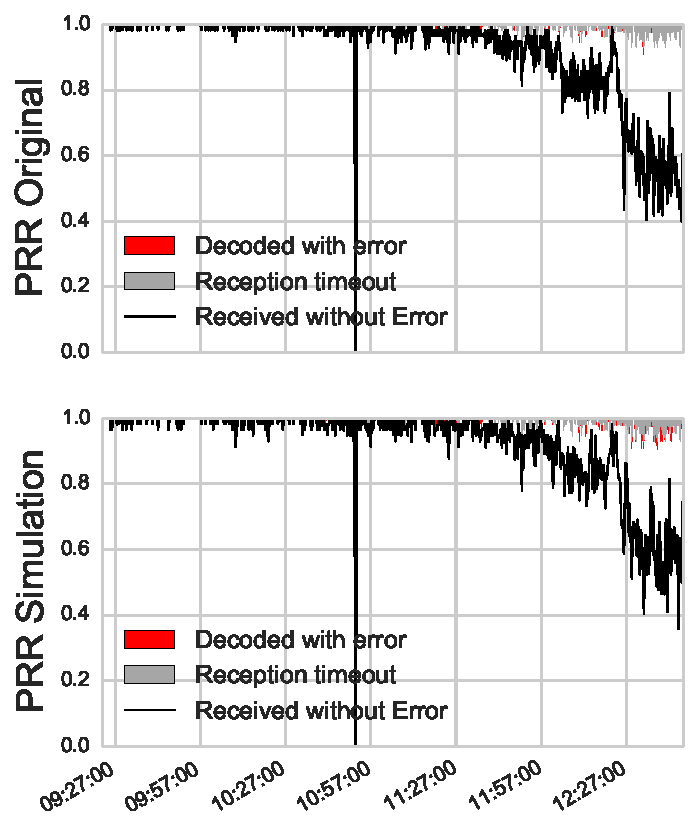
\includegraphics[width=0.475\columnwidth]{figures/fec_scheme_box0_box1_os_0-1_Throughput}
		\label{fig:prr_link_01_transmitter_fec}
	}
	\subfigure[Comparison of link~\ref{fig:prr_link_01_receiver}.] {
		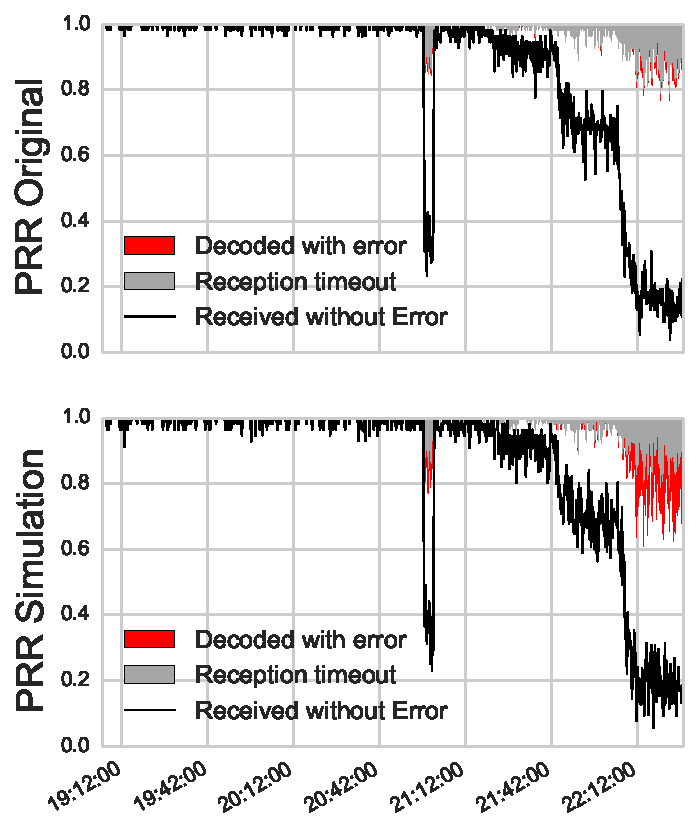
\includegraphics[width=0.475\columnwidth]{figures/fec_scheme_box1_box0_os_0-1_Throughput}
		\label{fig:prr_link_01_receiver_fec}
	}
	\caption{Original and simulated \acs{PRR} of the two $RS(80,70)$ encoded links of Figure~\ref{fig:prr_link_01}. Note the drop in simulated \acs{RS} decoded \acs{PRR} in (b).}
	\label{fig:prr_link_01_fec}
\end{figure}

\begin{figure}[t]
	\subfigure[Comparison of link~\ref{fig:prr_link_10_receiver}.] {
		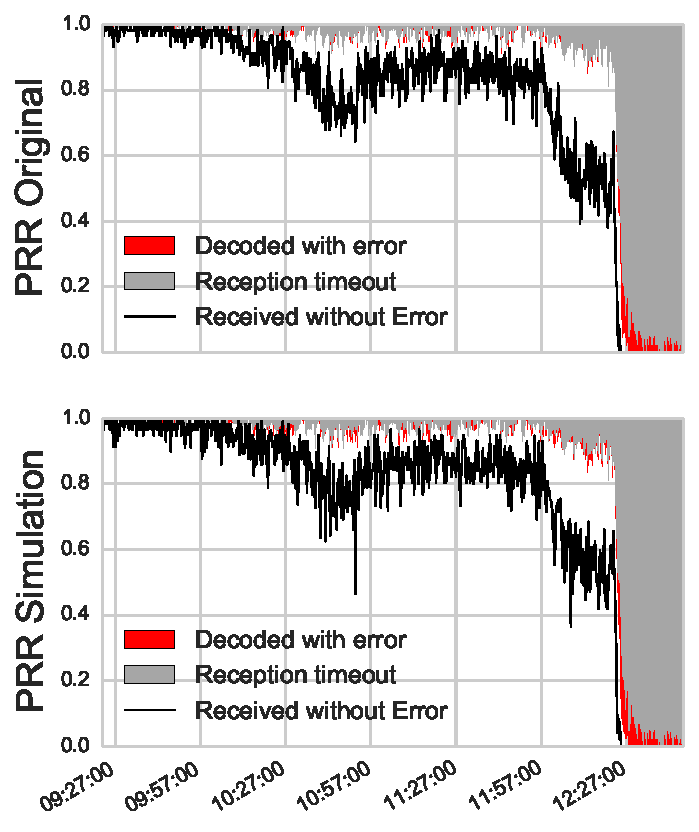
\includegraphics[width=0.475\columnwidth]{figures/fec_scheme_box0_box1_os_1-0_Throughput}
		\label{fig:prr_link_10_receiver_fec}
	}
	\subfigure[Comparison of link~\ref{fig:prr_link_10_transmitter}.] {
		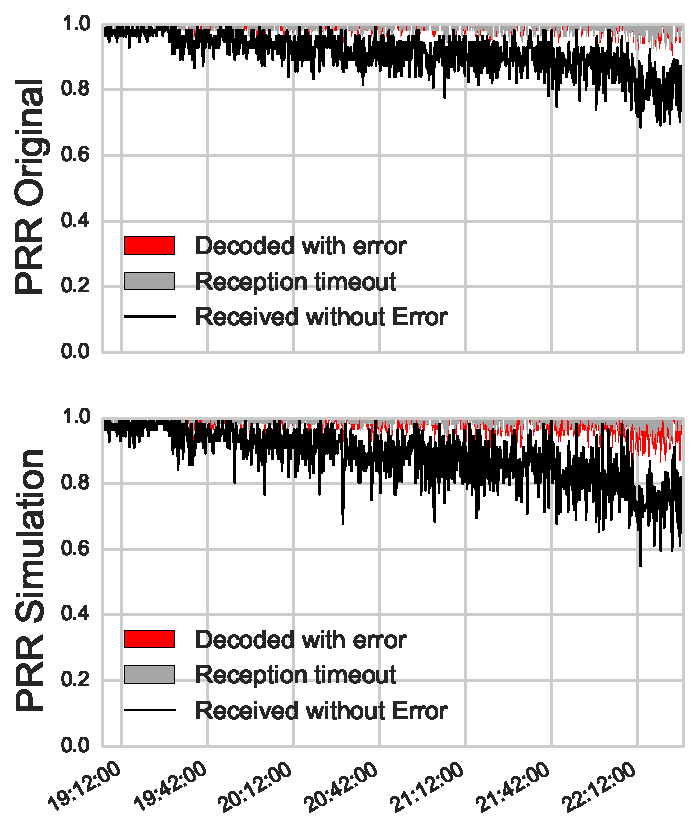
\includegraphics[width=0.475\columnwidth]{figures/fec_scheme_box1_box0_os_1-0_Throughput}
		\label{fig:prr_link_10_transmitter_fec}
	}
	\caption{Original and simulated \acs{PRR} of the two $RS(80,70)$ encoded links of Figure~\ref{fig:prr_link_10}.}
	\label{fig:prr_link_10_fec}
\end{figure}

These results show that this simple simulator is a very good time- and cost-saving alternative to testing the effects of different payloads over a real link, if good original data is available.
Using our trace-based simulator eliminates the effect of uncontrollable environmental factors or hardware issues on repeatability and allows us to focus purely on the message content, without assuming  idealized and monolithic link properties.


\section{Comparing \acs{RS} Scheme Strengths}

Our first idea was to keep a constant data size of $k=80$ and add parity bytes, making the entire message longer.
However, longer packets require more energy to transmit, a metric which has to be included somehow when comparing different $k$.
Furthermore, because of the size limit of the \ac{MPDU} of 127 bytes, of which 26 are already used, this only leaves $n=101$ bytes with a maximum of $n-k=19$ parity bytes, which would not allow to encode with more than 18\% coding overhead.
We could have split the message into two packets, however, this would have made it even harder to compare them, since now two packets must be received in the right sequence.

Therefore, we abandoned this idea and fit the entire encoded message into 80 bytes, including parity bytes as shown in Figure~\ref{fig:rs_codeword}.
This means we can only transfer $k$ bytes of encoded data, effectively reducing data rate while gaining robustness, which we want to use for a metric for comparing \ac{RS} performance.
We combine this reduction of data rate and the corruption of decoded packets as throughput, normalized over the number of \emph{received} messages.
We calculated the normalized throughput $T(80, k)$ using the following formula:

\[ T(80, k) = \frac{k}{80} \frac{PRR_{decoded}}{PRR_{received}} \]

This metric allows us to compare \ac{RS} performance not only between different coding strengths, but augment that comparison with context of the link's quality.
% The normalized throughputs of the original versus simulated links are also available in Figures~\ref{fig:prr_link_01_fec} and \ref{fig:prr_link_10_fec}.
% Especially the drop in Figure~\ref{fig:prr_link_01_receiver} visualizes the previous findings that the simulation slightly underestimates, but never overestimates \ac{RS} decoded \ac{PRR}.

For each of the four links discussed in Section~\ref{sec:packet_reception_rate} we simulated new $RS(80, k)$ encoded payload for $k$ in 10 byte increments up to $k=60$, then in 2 byte increments up to $k=78$.
We plotted the normalized throughputs $T(80, k)$ in Figure~\ref{fig:throughput_link_fec}, with the dashed line showing throughput without RS encoding.
The graphs illustrate that even using only 2 parity bytes at $k=78$ can already significantly improve \ac{PRR}, since most messages only have a few burst errors, and all those constrained to one byte can be corrected.

Adding two more parity bytes for $k=76$ improves \ac{PRR} even more, but only in a few areas.
From $k=74$ to $k=60$ no significant improvement shows, especially at low temperatures.
Using $k=60$ shows stability up to high temperature of $80\,^{\circ}\mathrm{C}$ in all Figures except \ref{fig:throughput_link_10_receiver_fec}.
At and below $k=50$ no improvement of throughput is visible except in Figure~\ref{fig:throughput_link_10_receiver_fec}, where $k=30$ and $k=20$ hold throughput the longest.

By comparing Figure~\ref{fig:prr_link_01_receiver_fec} and \ref{fig:throughput_link_01_receiver_fec}, we can deduct that in that link the simulated throughput above \SI{70}{\celsius} is actually worse than in reality. Therefore we can safely assume $k=60$ as stable at that temperature.

\begin{figure}[t]
	\subfigure[Simulated link~\ref{fig:prr_link_01_transmitter}.] {
		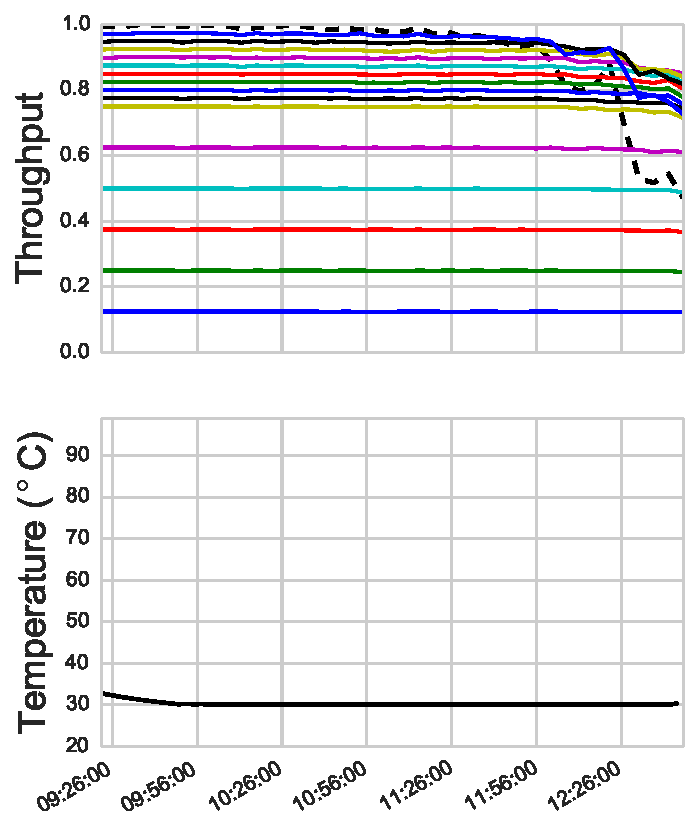
\includegraphics[width=0.475\columnwidth]{figures/fec_scheme_box0_box1_0-1_Throughput}
		\label{fig:throughput_link_01_transmitter_fec}
	}
	\subfigure[Simulated link~\ref{fig:prr_link_01_receiver}.] {
		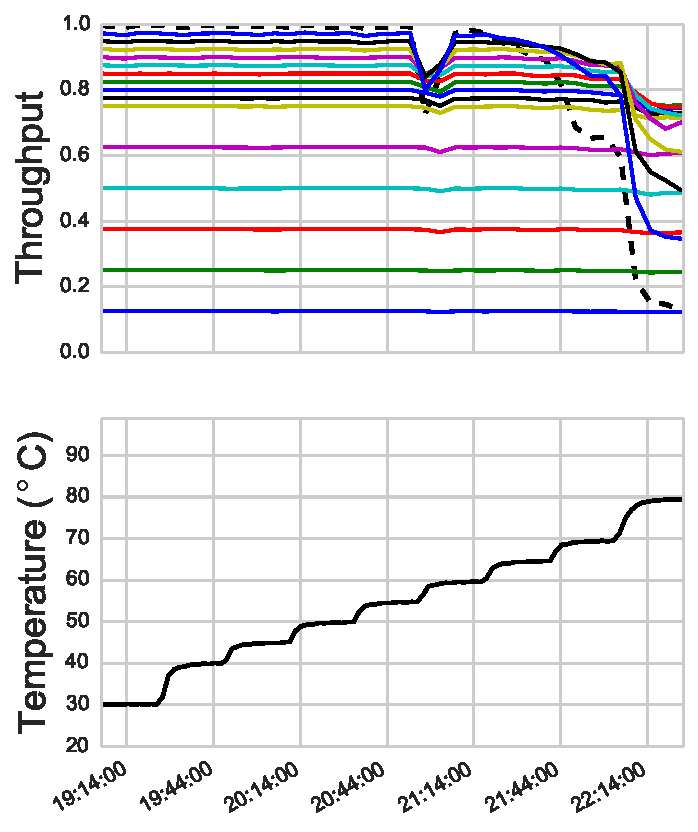
\includegraphics[width=0.475\columnwidth]{figures/fec_scheme_box1_box0_0-1_Throughput}
		\label{fig:throughput_link_01_receiver_fec}
	}
	\subfigure[Simulated link~\ref{fig:prr_link_10_receiver}.] {
		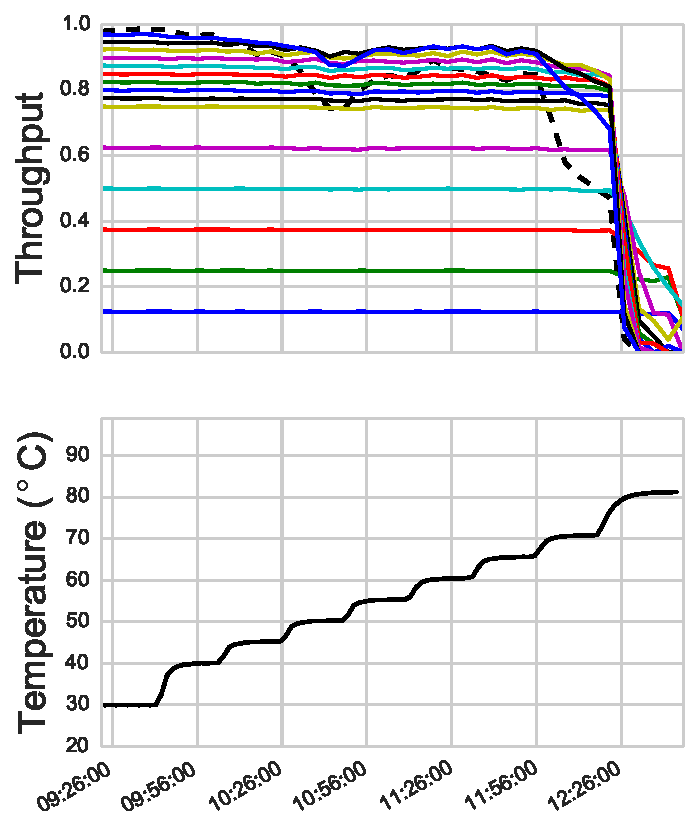
\includegraphics[width=0.475\columnwidth]{figures/fec_scheme_box0_box1_1-0_Throughput}
		\label{fig:throughput_link_10_receiver_fec}
	}
	\subfigure[Simulated link~\ref{fig:prr_link_10_transmitter}.] {
		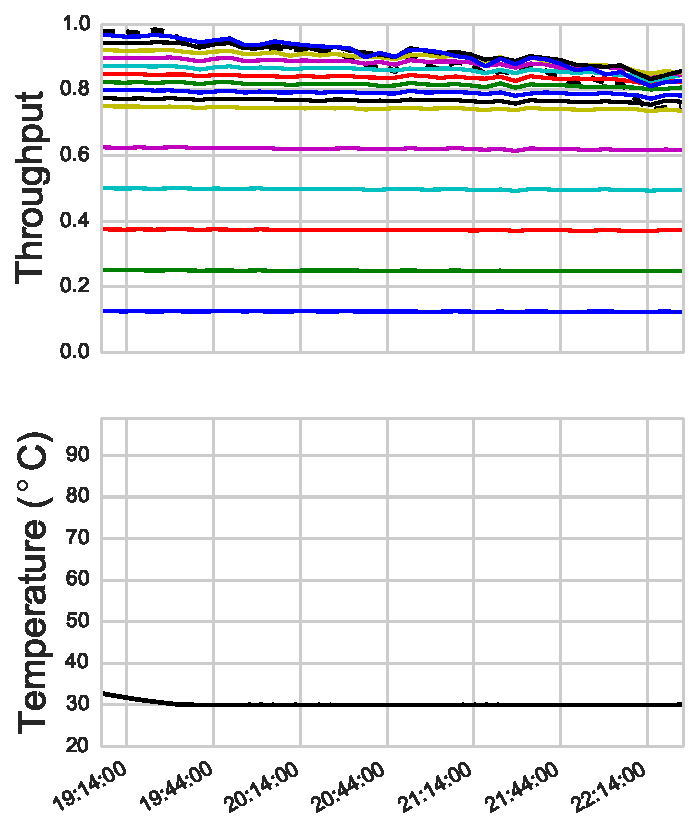
\includegraphics[width=0.475\columnwidth]{figures/fec_scheme_box1_box0_1-0_Throughput}
		\label{fig:throughput_link_10_transmitter_fec}
	}
	\caption{Comparison of throughputs $T(80, k)$ of all four simulated links of Section~\ref{sec:packet_reception_rate} for \\$k \in \{10,20,30,40,50,60,62,64,66,68,70,72,74,76,78\}$ over temperature. The dashed line shows throughput at $k=80$, which is equivalent to using no parity bytes.}
	\label{fig:throughput_link_fec}
\end{figure}



\section{Discussion}

Considering that the goal of using an \ac{FEC} in the context of low power networks such as \ac{WSN}s is to maximize energy efficiency of communications, we are not only looking for the $k$ with maximum throughput, but also with the least retransmissions.
We also have to consider that the link quality can already be poor at low temperature, therefore using no parity bytes at low temperatures is not a good idea either.

As per our findings, we propose one possible \ac{RS} scheme starting with $k=70$, which is 12.5\% overhead (the same as the popular $RS(255,223)$~\cite{Ma2009}), at low temperatures and linearly increase this to $k=60$ (or 25\% overhead) as receiver temperature increases to $70\,^{\circ}\mathrm{C}$ and above.
Starting with $k=70$ will give some protection against a random decrease in link quality as seen in Figure~\ref{fig:throughput_link_01_receiver_fec}.
In cases of extremely high bit error, such as in Figure~\ref{fig:throughput_link_10_receiver_fec}, we can still regain some throughput by using $60-80\%$ coding overhead with $k=30$ or $k=20$.
However, considering the extremely low \ac{PRR} in this area (compare with Figure~\ref{fig:prr_link_10_receiver_fec}), most of these messages will likely never be received anyway, which makes this option only viable when communication at these temperatures is absolutely necessary.

The results of Boano~\etal~\cite{Boano2013} strongly suggested that the loss in \ac{PRR} is more pronounced when heating the transmitter than the receiver.
This would have allowed us to use local temperature measurements to adapt the coding strength of our \ac{FEC} scheme to counteract the loss in \ac{PRR}.
Unfortunately, our results firmly oppose the findings of Boano~\etal{}: heating the receiver creates a higher loss in \ac{PRR} than heating the transmitter, therefore making such an approach unusable.
However, using temperature as another source for assessing link quality has the distinct advantage of being always available on the receiver locally, compared to \ac{LQI} and \ac{RSSI}, which requires a message to be received first.

We therefore propose another solution to adapt \ac{FEC} strength:
the receiver should monitor its local temperature and send out a warning broadcast to all potential transmitters, before its temperature becomes too high.
The transmitters can then address this mote with the appropriate \ac{FEC} strength.
The advantage of this active, preemptive approach over backchanneling link quality information is that in setups where transmissions only occur sparsely, a ``test'' transmission to judge link quality is not required.





%%%%%%%%%%%%%%%%%%%%%%%%%%%%%%%%%%%%%%%%%%%%%%%%%%%%%%%%%%%%%
%% LITERATUR UND ANDERE VERZEICHNISSE
%%%%%%%%%%%%%%%%%%%%%%%%%%%%%%%%%%%%%%%%%%%%%%%%%%%%%%%%%%%%%
%% Ein kleiner Abstand zu den Kapiteln im Inhaltsverzeichnis (toc)
\ifnotdraft{
\addtocontents{toc}{\protect\vspace*{\baselineskip}}
\cleardoublepage
%% Literaturverzeichnis
\phantomsection % phantomsection wird benötigt, damit z.B. hyperref die richtige Seite verlinkt.
\addcontentsline{toc}{chapter}{Bibliography}
%\nocite{*} %Auch nicht-zitierte BibTeX-Einträge werden angezeigt.
\bibliography{literature/literature}%Eine Datei 'literatur.bib' wird hierfür benötigt.
\bibliographystyle{acmurl}%Art der Ausgabe: plain / apalike / amsalpha / ...
}

%% Abbildungsverzeichnis
%\clearpage
%\addcontentsline{toc}{chapter}{List of Figures}
%\listoffigures

%% Tabellenverzeichnis
%\clearpage
%\addcontentsline{toc}{chapter}{List of Tables}
%\listoftables


%%%%%%%%%%%%%%%%%%%%%%%%%%%%%%%%%%%%%%%%%%%%%%%%%%%%%%%%%%%%%
%% ANHÄNGE
%%%%%%%%%%%%%%%%%%%%%%%%%%%%%%%%%%%%%%%%%%%%%%%%%%%%%%%%%%%%%
\appendix
\chapter{Appendix}

\section{List of Abbreviations}

\begin{acronym}[MOSFET]
	\setlength{\itemsep}{-\parsep}
	
	\acro{MOSFET}{Metal–Oxide–Semiconductor Field-Effect Transistor}
	\acro{ISP}{In-System Programming}
	\acro{PRR}{Packet Reception Rate}
	\acro{PID}{Proportional-Integral-Derivative}
	\acro{ATX}{Advanced Technology eXtended}
	\acro{DCO}{Digitally Controlled Oscillator}
	\acro{UART}{Universal Asynchronous Receiver Transmitter}
	\acro{BER}{Bit Error Rate}
	\acro{LQI}{Link Quality Indication}
	\acro{RSSI}{Received Signal Strength Indication}
\end{acronym}


\begin{table}
	\subtable[Average Packet Reception Rate in \%]
	{
		\begin{tabularx}{\linewidth}{|c*{4}{|d{-1}}|}
		\hline
		\T \cellcolor{slightgray} Receiver	& \multicolumn{1}{X|}{\cellcolor{motered} \centering Sender 0} & \multicolumn{1}{X|}{\cellcolor{motered} \centering Sender 1} & \multicolumn{1}{X|}{\cellcolor{moteblue} \centering Sender 2}	& \multicolumn{1}{X|}{\cellcolor{moteblue} \centering Sender 3}\\
		\hline

		\cellcolor{moteblue}\T 4 & \cellcolor{slightred} 3.2  & \cellcolor{slightgreen} 96.9 & \cellcolor{slightred} 5.5  & \cellcolor{slightgreen} 100.0 \B\\
		\hline
		\cellcolor{motered}\T 5 & 81.9 & 87.2 & \cellcolor{slightred} 0.4  & \cellcolor{slightgreen} 99.2 \B\\
		\hline
		\cellcolor{moteblue}\T 6 & \cellcolor{slightgreen} 98.1 & 75.2 & 89.9 & \cellcolor{slightred} 0.1  \B\\
		\hline
		\cellcolor{motered}\T 7 & \cellcolor{slightgreen} 96.2 & \cellcolor{slightred} 2.0    & 57.3 & 44.0	\B\\
		\hline 
		\end{tabularx}
	}

	\subtable[Average Error Free Packets Reception Rate in \%]
	{
		\begin{tabularx}{\linewidth}{|c*{4}{|d{-1}}|}
		\hline
		\T \cellcolor{slightgray} Receiver	& \multicolumn{1}{X|}{\cellcolor{motered} \centering Sender 0} & \multicolumn{1}{X|}{\cellcolor{motered} \centering Sender 1} & \multicolumn{1}{X|}{\cellcolor{moteblue} \centering Sender 2}	& \multicolumn{1}{X|}{\cellcolor{moteblue} \centering Sender 3}\\
		\hline

		\cellcolor{moteblue}\T 4 & \cellcolor{slightred} 0.0  & 69.5 & \cellcolor{slightred} 2.7  & \cellcolor{slightgreen} 100.0 \B\\
		\hline
		\cellcolor{motered}\T 5 & \cellcolor{slightred} 7.1 & 10.8 & \cellcolor{slightred} 0.0  & 88.3 \B\\
		\hline
		\cellcolor{moteblue}\T 6 & 83.8 & \cellcolor{slightred} 2.1 & 22.1 & \cellcolor{slightred} 0.0  \B\\
		\hline
		\cellcolor{motered}\T 7 & \cellcolor{slightgreen} 96.0 & \cellcolor{slightred} 0.1    & \cellcolor{slightred} 9.8 & \cellcolor{slightred} 1.4	\B\\
		\hline 
		\end{tabularx}
	}

	\subtable[Average LQI values]
	{
		\begin{tabularx}{\linewidth}{|c*{4}{|d{-1}}|}
		\hline
		\T \cellcolor{slightgray} Receiver	& \multicolumn{1}{X|}{\cellcolor{motered} \centering Sender 0} & \multicolumn{1}{X|}{\cellcolor{motered} \centering Sender 1} & \multicolumn{1}{X|}{\cellcolor{moteblue} \centering Sender 2}	& \multicolumn{1}{X|}{\cellcolor{moteblue} \centering Sender 3}\\
		\hline

		\cellcolor{moteblue}\T 4 & \cellcolor{slightred} 50 & 79 & \cellcolor{slightred} 77 & \cellcolor{slightgreen} 101 \B\\
		\hline
		\cellcolor{motered}\T 5 & 71 & 72 & \cellcolor{slightred} 49  & 87 \B\\
		\hline
		\cellcolor{moteblue}\T 6 & 85 & 67 & 73 & \cellcolor{slightred} 35  \B\\
		\hline
		\cellcolor{motered}\T 7 & \cellcolor{slightgreen} 106 & \cellcolor{slightred} \cellcolor{slightred} 44 & 65 & 61	\B\\
		\hline 
		\end{tabularx}
	}

	\caption{Complete table of link qualifiers from the experiment described in Subsection~\ref{subsec:effects_of_board_layout}. Good links (PRR > 90\%) are marked green, bad links (PRR < 10\%) red. Notice the distinction between PRR in Table (a) and \emph{error-free} PRR in Table (b) in comparison to LQI in Table (c).}

	\label{tab:8mote_link_qualities}
\end{table}

\end{document}
